% Use only LaTeX2e, calling the article.cls class and 12-point type.

\documentclass[12pt]{article}

% Users of the {thebibliography} environment or BibTeX should use the
% scicite.sty package, downloadable from *Science* at
% www.sciencemag.org/about/authors/prep/TeX_help/ .
% This package should properly format in-text
% reference calls and reference-list numbers.

%\usepackage{scicite}
\usepackage{multirow}
\usepackage{graphicx}
\usepackage{amsmath,array,mathtools}
\usepackage{color,soul}
\usepackage[toc,page]{appendix}
\usepackage[symbol]{footmisc}

% Use times if you have the font installed; otherwise, comment out the
% following line.

\usepackage{times}

% The preamble here sets up a lot of new/revised commands and
% environments.  It's annoying, but please do *not* try to strip these
% out into a separate .sty file (which could lead to the loss of some
% information when we convert the file to other formats).  Instead, keep
% them in the preamble of your main LaTeX source file.


% The following parameters seem to provide a reasonable page setup.

\topmargin 0.0cm
\oddsidemargin 0.2cm
\textwidth 16cm 
\textheight 21cm
\footskip 1.0cm


%The next command sets up an environment for the abstract to your paper.

\newenvironment{sciabstract}{%
\begin{quote} \bf}
{\end{quote}}


% If your reference list includes text notes as well as references,
% include the following line; otherwise, comment it out.

\renewcommand\refname{References and Notes}

% The following lines set up an environment for the last note in the
% reference list, which commonly includes acknowledgments of funding,
% help, etc.  It's intended for users of BibTeX or the {thebibliography}
% environment.  Users who are hand-coding their references at the end
% using a list environment such as {enumerate} can simply add another
% item at the end, and it will be numbered automatically.

\newcounter{lastnote}
\newenvironment{scilastnote}{%
\setcounter{lastnote}{\value{enumiv}}%
\addtocounter{lastnote}{+1}%
\begin{list}%
{\arabic{lastnote}.}
{\setlength{\leftmargin}{.22in}}
{\setlength{\labelsep}{.5em}}}
{\end{list}}


% Include your paper's title here

\title{Energy and Time Determine Scaling in \\Biological and Computer Designs} 
%Biological and Computer Designs Minimize Energy and Time.  

% Place the author information here.  Please hand-code the contact
% information and notecalls; do *not* use \footnote commands.  Let the
% author contact information appear immediately below the author names
% as shown.  We would also prefer that you don't change the type-size
% settings shown here.

\author
{Melanie Moses,$^{1,2,3\ast}$ Stephanie Forrest$^{1,2,3}$ George Bezerra,$^{1}$ \\Benjamin Edwards$^{1}$, James Brown,$^{2,3}$ \\
\\
\normalsize{$^{1}$Department of Computer Science}\\
\normalsize{University of New Mexico, Albuquerque, NM, USA.}\\
\normalsize{$^{2}$Department of Biology}\\
\normalsize{The University of New Mexico, Albuquerque, NM, USA.}\\
\\
\normalsize{$^{3}$The Santa Fe Institute, Santa Fe, NM, USA.}\\
\\
\normalsize{$^\ast$To whom correspondence should be addressed}\\
\normalsize{E-mail: melaniem@cs.unm.edu}\\
\normalsize{Address: Department of Computer Science}\\
\normalsize{1 University of New Mexico, Albuquerque, NM USA}\\
\normalsize{Phone: 505-277-3112}\\
}



% Include the date command, but leave its argument blank.

\date{\normalsize{{\bf Keywords:} network scaling, power consumption, 
metabolic rate, complex systems, energy-time product, organism, 
computer chip}\\
\normalsize{{\bf Classification:} Major: ; Minor: }}



%%%%%%%%%%%%%%%%% END OF PREAMBLE %%%%%%%%%%%%%%%%



\begin{document} 

\newcounter{casenum}
\newenvironment{caseof}{\setcounter{casenum}{1}}{\vskip.5\baselineskip}
\newcommand{\case}[2]{\vskip.5\baselineskip\par\noindent {\bfseries Case
\arabic{casenum}:} #1: #2\addtocounter{casenum}{1}}

% Double-space the manuscript.

\baselineskip24pt

% Make the title.

\maketitle 


\newpage

% Place your abstract within the special {sciabstract} environment.
% \centerline{\Large{\bf Abstract}}
% \begin{sciabstract}
% Metabolic rate in organisms and power consumption in computers are 
% analogous quantities that scale similarly with size.  We analyze 
% organisms and computer chips as systems in which natural selection or 
% human engineering has produced optimized networks that minimize the 
% energy-time product.  The network designs simultaneously reduce energy 
% costs and increase flow rates.  Using a simple network model, our 
% analysis explains empirically observed trends in the scaling of 
% metabolic rate in organisms and power consumption in chips across 
% several orders of magnitude in size.  This result suggests that a 
% single principle governs the designs of many complex systems that 
% process energy, materials, and information.
% \end{sciabstract}

% Place your abstract within the special {sciabstract} environment.
% The new abstract
\centerline{\Large{\bf Abstract}}

\begin{sciabstract}

  Metabolic rate in animals and power consumption in computers are analogous
  quantities that scale similarly with size.  We analyze vascular systems of
  vertebrates and on-chip networks of microprocessors, where natural selection
  and human engineering respectively have produced networks that minimize both energy dissipation
  and delivery times.   
 % energy time product.  Both network designs simultaneously reduce energy costs
  %and increase flow rates.  
  Using a simple network model that simultaneously minimizes the energy time product, our analysis explains
  empirically observed trends in the scaling of metabolic rate in organisms and
  power consumption and performance in chips across several orders of magnitude
  in size.  This result suggests that a single principle governs the designs of
  many complex systems that process energy, materials, and information. Just as
  the evolutionary transitions in biology are associated with shifts in
  metabolism, so do our models suggest that energy efficiency will change
  as computer designs transition to decentralized multi-core and
  distributed cyber-physical systems.

\end{sciabstract}

\newpage

\section{Introduction}
\label{sec:intro}

Both organisms and computers have evolved from relatively simple beginnings
into complex systems that vary by orders of magnitude in size and number of
components. Evolution, by natural selection in organisms and by human
engineering in computers, required critical features of architecture and
function to be scaled up as size and complexity increased. In biology,
Kleiber's law describes the empirical relation between metabolic rate and many
other traits, such as lifespan, heart rate, and number of offspring, with body
size \cite{kleiber47}.  Similarly, computer architecture has Moore's law to
describe scaling of transistor density and performance \cite{moore98}, Koomey's
law for the energy cost per computation \cite{koomey11}, and Rent's rule for
the external communication per logic block \cite{christie00}.

% We posit that these empirical patterns originate from a common 
% principle: Networks that deliver resources are optimized to reduce 
% energy dissipation and increase flow rates, expressed here as 
% minimizing the energy-time product. {\bf Need to clarify where energy
%   is disipated.  we ention energy-time product but rest of paragraph
%   is about the network and not the nodes.}  In biology, the vascular network 
% of vertebrate animals supplies oxygen and nutrients to every cell, 
% fueling metabolism for maintenance, growth and reproduction.  Since 
% energy is a limited resource, organisms are selected to minimize the 
% energy dissipated in the network \cite{west97}. Similarly, computation 
% in microprocessors relies on a network of microscopic wires that 
% transmits bits of information between transistors on a chip.  In order 
% to maximize computer performance and minimize power consumption, this 
% network is designed to deliver the maximum information flow at the 
% lowest possible energy cost.

We posit that these empirical patterns originate from a common principle:
Networks that deliver resources are optimized to reduce energy dissipation and
increase flow rates, expressed here as minimizing the energy-time product. That
is, both living systems and computer chips are designed to maximize the rate at
which resources are delivered to terminal nodes of a network and to minimize
the energy dissipated as it is delivered.  For example, in biology the vascular network of vertebrate
animals supplies oxygen and nutrients to every cell, fueling metabolism for
maintenance, growth and reproduction.  Since energy is a limited resource, we
assume that organisms are selected to maximize the delivery rate of oxygen while minimizing the energy that is dissipated as oxygen is delivered through the network \cite{west97} and processed to produce ATP in the mitochondria. Similarly, computation in microprocessors relies on a
network of microscopic wires that transmits bits of information between
transistors on a chip.  In order to maximize computation speed and minimize
power consumption, this network is designed to deliver the maximum information
flow at the lowest possible energy cost.

Here, we model vertebrates as composed of regions of tissue that receive oxygen
carried by blood via a hierarchical vascular network of pipes, and we model
microprocessors as composed of transistors that perform computation, exchanging
information over a network of wires.  As each system scales up in size,
we consider: 1) the rate at which resources are delivered by the network and
processed in the nodes; and 2) the energy dissipated during these processes.
Despite the obvious differences between organisms and chips, we present a
general model and derive energy and time scaling relations from physical
principles applicable to each system. Using these relations, we express the
optimal network design as a trade-off between energy cost and processing speed. 

% Here, we model vertebrates as composed of regions of tissue that 
% receive blood via a hierarchical vascular network of pipes, and we 
% model microprocessors as composed of transistors that perform 
% computation, exchanging information over a modular network of wires.  
% As each system scales up in size, we consider: 1) the time for 
% resources to flow through the network and be processed in the nodes; 
% and 2) the energy dissipated during these processes. Despite the 
% obvious differences between organisms and chips, we derive general 
% energy and time scaling relations from physical principles applicable 
% to each system. Using these relations, we express the optimal network 
% design as an energy-time product minimization problem.

Previous biological scaling models have sought either to minimize energy dissipation, e.g.,~\cite{west97} or to maximize resource delivery rate~\cite{banavar10}, but they have
not formalized the trade-offs between these goals, as we do here.  This formalization
helps explain how nature and engineering are able to produce designs that
approach pareto-optimality along the energy-time trade-off.  Thus, in biology
evolution has produced mammals ranging in size from mice to elephants, rather
than converging on a single optimal size, and in computer architecture
engineers have designed processors ranging from thousands to
billions of transistors, each of which fills a specific computational niche.

In the rest of the paper, we present the unified model of network scaling
(Section~\ref{sec:unified-model}) and the basic assumptions underlying the
model (Section~\ref{sec:assumptions}).  We then use the model to derive a
series of predictions about how time and energy scale with system size, first
for organisms (Section~\ref{sec:organisms}) and then for computers
(Section~\ref{sec:computers}). We then discuss new insights into previously
analyzed scaling relationships in biology that we gain from the time-energy
minimization framework, and we test our scaling predictions with empirical
power and performance data on computer chips.  Finally, in Section~\ref{sec:discussion}  we discuss the implications of these results for
evolutionary transitions in nature and engineering.

\begin{figure}[!h]
\centering
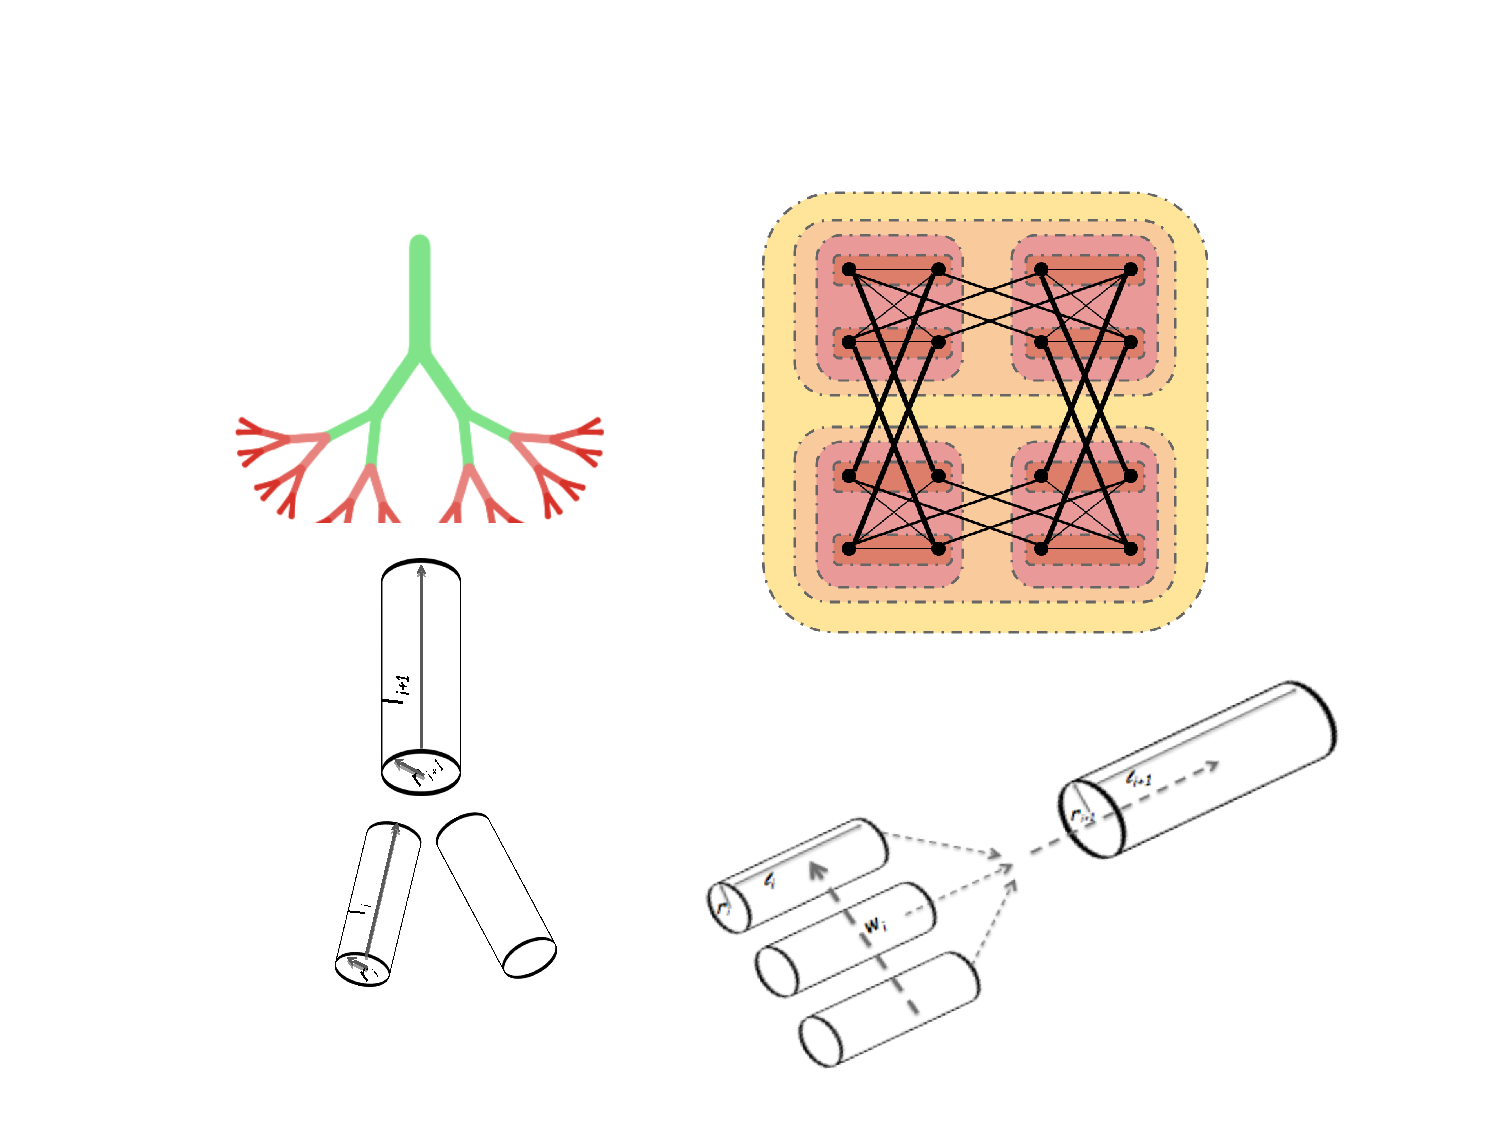
\includegraphics[height=90mm]{Figures/Figure1RoyalSocietyDraft2.pdf}
\label{fig:firstfig}

<<<<<<< HEAD
\caption{Idealized branching models in biology (A and B) and computers (C and D). Panel A shows a bifurcating cardiovascular tree ($\lambda = 2$) with  $H = 6$ hierarchical levels and $N = 32$ terminal branches of radius $r_0$ and length $l_0$. $D_r$ defines the relative radius of pipes between successive branches; $D_r = 2$ in the upper (green) branches the network so that the summed cross sectional area at each level is equal; such area-preserving branching results in constant velocity through the pipes. In the lower (red) branches, $D_r = 2.5$; such area increasing branching slows velocity at each bifurcation. $D_l$ defines both the physical dimension filled by the system and the relative length of pipe between successive hierarchical levels ($D_l = 3$ in 3-dimensional organisms but the 2-dimensional figure shows $D_l = 2$). Panel B shows the radius and length of successive branches. Panel C shows the semi-hierarchical branching of logic wires on a computer chip. Wire length and radius scaling are shown with $D_r = D_l = 2$.  $D_w$ defines how the ratio of internal (intra-module) communication per node to external (inter-module) communication per node scales with the level of the module in the hierarchy. Each module within a hierarchical level is shaded the same color. Here, $D_w = 2$ so that the probability of a wire connecting to each node within a module doubles with each hierarchical level. Panel D shows the radius, length and relative communication between successive branches.}
=======
\caption{Idealized branching models in biology (A and B) and computers (C and
D). Panel A shows an example of a bifurcating cardiovascular tree ($\lambda =
2$) with  $H = 6$ hierarchical levels and $N = 32$ terminal branches of radius
$r_0$ and length $l_0$. $D_r$ defines the relative radius of pipes between
successive branches; $D_r = 2$ in the upper (green) branches the network so
that the summed cross sectional area at each level is equal; such
area-preserving branching results in constant velocity through the pipes. In
the lower (red) branches, $D_r = 2.5$; such area increasing branching slows
velocity at each bifurcation. $D_l$ defines the relative length of pipe between
successive hierarchical levels ($D_l = 3$ in organisms but for simplicity the
figure shows $D_l = 2$. Panel B shows the radius and length of successive
branches. Panel C shows the semi-hierarchical branching of logic wires on a
computer chip. Wire length and radius scaling are shown with $D_r = D_l = 2$.
$D_w$ defines how the ratio of internal (intra-module) communication per node
to external (inter-module) communication per node scales with the level of the
module in the hierarchy. Each module within a hierarchical level is shaded the
same color. Here, $D_w = 2$ so that the probability of a wire connecting to
each node within a module doubles with each hierarchical level. Panel D shows
the radius, length and relative communication between successive branches.}
>>>>>>> origin/master

%\caption{Idealized branching models in biology and computers.
%  $lambda$ is the branching factor (e.g., $lambda$ is 2 in panel A); $H$ is the number
%  of hierarchical levels in the network; $N$ is the number of terminal
%  nodes in the network. $D_l$ defines the relative length of pipe
%  between successive hierarchical levels; $D_r$ defines the relative
%  radius of pipes between successive hierarchical levels of the
%  network; and $D_w$ (panel B only) defines how
%  the ratio of internal (intra-module) communication per node to external
%(inter-module) communication per node scales with the level of the module in
%the hierarchy. Panel A shows hierarchical fractal branching of the cardiovascular
%  network, and Panel B illustrates the semi-hierarchical branching of
%  a wire networks on a chip.  FIXME(Keep c and d?) }

\end{figure}
\section{Unified Model of Network Scaling}
\label{sec:unified-model}


Vascular systems are hierarchical branching networks where blood vessels
(pipes) become thicker and longer through the hierarchy from the capillaries
to the aorta. Similarly, microprocessor chips are organized hierarchically into
a nested structure of modules and submodules, where wires become longer and
thicker as the hierarchical level of a module increases
(Figure~\ref{fig:firstfig}).  These wires are organized into metal
layers, where short, thin wires are routed on the lowest layers, and long,
thick wires are placed on the top layers. We model the scaling of length ($l$)
and thickness ($r$) of both pipes and wires as

\begin{equation}
l_i = l_0 \lambda^{\frac{i}{D_l}}
\end{equation}

\noindent and

\begin{equation}
  r_i = r_0 \lambda^{\frac{i}{D_r}},
\label{eq:rscaling}
\end{equation}

\noindent where $i$ is the hierarchical level of a branch or module, $\lambda$
is the branching factor, and $D_l$ and $D_r$ are the length and thickness
dimensions. This model is akin to the hierarchical pipe model of vascular
systems proposed in \cite{west97}, and $\lambda^{\frac{1}{Dr}}$ and
$\lambda^{\frac{1}{Dl}}$ correspond to West et al.'s $\beta$ and $\gamma$
respectively (note that in~\cite{west97}, the aorta or top of the network is
labelled as level 0, while here the smallest branches, the capillaries, are
labelled as level 0.)
% where $l_i$ ROUGHLY corresponds to $\gamma$
%and $r_i$ ROUGHLY corresponds to $\beta$.  
In vascular networks, $r$ represents the radius of cylindrical pipes, and in
computer interconnect, $r$ represents the width of wires with aspect ratio 1.
$D_r$ describes the relative radius of pipes between successive hierarchical
levels.  The smallest edges occur at $i = 0$, and have constant radius, $r_0$,
and length, $l_0$, that scales with system size~\cite{banavar10}. 

%\begin{figure}
%\caption{Schematic: Panel c illustrates the communication dimension, $D_w$,
%  which measures how the ratio of internal (intra-module) communication per node to
%  external (inter-module) communication per node scales with the level of the module in
%  the hierarchy. Note, that if we had a biological version, we would
%  have MORE edges.}
%  \label{fig:model-schematic}
%\end{figure}

The length parameter $D_l$ is determined by the spatial dimension occupied by the
nodes of the network~\cite{mandelbrot83}.  For chips, $D_l = 2$, since
transistors are placed on a single two-dimensional layer~\cite{donath81}. For
three-dimensional organisms,  $D_l = 3$. Based on the argument that the length of a vessel defines the radius of a 3-dimensional volume of tissue supplied by that vessel, each successive vessel in the hierarchy scales according to Eq. 1 with $D_l = 3$~\cite{west97, banavar10}. Similarly, the length of each successive wire on a 2-dimensional chip defines an area to which that wire delivers bits~\cite{moses08}. Thus, in the simplest networks that efficiently deliver resources homogeneously throughout a volume or area, $D_l$ describes both the relative length of pipe between successive hierarchical levels and the physical
dimension of the system. For example in Figure \ref{sec:unified-model} C, where $\lambda = D_l = 2$, wires are $2^{1/2}$ times longer when they connect to successively higher modules in the hierarchy.

%FIXME: Move this to later: However,~\cite{newberry2015testing} find little empirical evidence for $D_l = 3$ in mouse vasculature, suggesting that the volume filling assumption may be oversimplified. 

Digital circuits scale in a third way beyond length and radius, which
has no direct analog in organisms.  In vascular networks, each pipe
branches at each hierarchical level forming a tree structure
(in the simplest case with $\lambda = 2$ forming
a binary tree.) Chips, however, have many cross connections at each
level of the network, and these cross connections
vary systematically with the hierarchical level.  Thus,
digital circuits are partially \emph{decentralized}, with networks
that connect
multiple sources and destinations, while vascular networks are
centralized, with blood flowing from a single heart. To account for
this difference, we introduce a new equation, in which the
communication (or number of wires) per module increases with the
hierarchical level as:  

\begin{equation}
  w_i = w_0 \lambda^{\frac{i}{D_w}},
\label{eq:communication}
\end{equation}

\noindent where $D_w$ is the communication dimension and $w_0$ is the average
number of wires per node.  This hierarchical scaling of communication is a
well-known pattern in circuit design called Rent's rule \cite{christie00},
where $p = \frac{1}{D_w}$ is the Rent's exponent.\footnote{Rent's rule is typically
  expressed as $C(n) = kn^p$, where $C_n$ is the external communication of a
  module, $n$ is the size of the module (number of nodes), $k$ is the average
  external communication of a module with size 1, and $p$ is the Rent's
  exponent. For a hierarchy with branching factor of $\lambda$, the size of a
  module is given as $n = \lambda^i$, where $i$ is the hierarchical level.
  Therefore, we can rewrite Rent's rule as $c_i = c_0 \times \lambda^{ip}$,
where $c_0 = w_0$ and $p = \frac{1}{D_w}$.} This pattern is not unique to circuits
and has been shown to occur in many biological networks
\cite{reda09,bassett10}.   Vascular systems correspond to a special case where 
%$w_0 = 1$ and $1/D_w = 0$, such that 
$w_i = 1$ for all $i$. 

\subsection{Assumptions of the Unified Model}
\label{sec:assumptions}

Before deriving scaling predictions, we state the
assumptions of the model and how they relate to earlier models, both in
computation and biology:

\begin{enumerate}
\item {\bf Time and energy are equally important constraints:} 
  System designs seek to deliver the maximum amount of
  resource per unit time for the minimum amount of energy overhead. 
%interpreted as minimizing the energy dissipated to deliver
%  and process a unit of resource, while simultaneously minimizing the
%  time to deliver and process that resource.  
  In computer architecture this relationship is expressed as the
  \emph{energy-delay product}, which formalizes the insight that a
  chip that is ten times faster or ten times more energy efficient is
  ten times better. 
%It is
%unrealistic that either of these quantities is minimized independently
%of the other.
%WHY ISN'T IT ADDITIVE?
% A multiplicative decrease of either quantity should be reflected
% proportionally by the energy-delay equation.  i.e., a chip that is
% 10 times faster, should make the energy-delay equation 10 times
% better.  Has something to do with multiplicity of components.

\item {\bf Steady state}: Resource supply matches processing
  demand~\cite{banavar10}.  That is, the network supplies resources continually
  to the nodes and is always filled to capacity.  This avoids network
  delays and the need to store resources in the system. Specifically,

  \begin{enumerate}

\item System designs balance network delivery rates with node processing
  speeds, so that resources are delivered at exactly the same rate that they
  are processed.

\item Pipelining: A concept from computer architecture in which resources,
  e.g., computer instructions, leave the source at the same rate that they are
  delivered to the terminal nodes, and the network is always full.  In the
  hierarchical networks considered here, the source is the highest branch
  %(root), 
  and the principle holds within every level of the hierarchy.
  Consequently, resources flow through the network continually %at maximum speed,
  without bottlenecks and they do not accumulate at source, sink, or intermediate locations.
  \end{enumerate}

\item {\bf Terminal units and service volumes:} In contrast to
  Ref.~\cite{west97} we do not assume that terminal units have fixed size.   In
  chips it is well known that transistor size has shrunk over many orders of
  magnitude over the past 50 years.   Previous scaling models of biology posit that the service volume
  (region served by terminal units of the network) actually increases with
  system size~\cite{west97,banavar10}.  Following Ref.~\cite{banavar10}, we
  assume that capillaries have fixed radius but that their length is
  proportional to the radius of the service volume.   Similarly, the radius of
  the isochronic region (service volume) for chips scales proportionally with
  decreasing transistor size.
% really we mean 'length' of one side of the transistor, aka process size.
\end{enumerate}

In addition to these general assumptions, we make the following
refinements to accommodate salient differences between biology and computer architecture.
\begin{enumerate}
\item In biology, the energy processed by a service volume,
  $E_{node}$, is invariant with system size. That is, as the service volume
  increases with body size, the total amount of energy processed
  remains constant.   We do not make this assumption for chips.

\item Component packing: In chips, we assume that total chip area is constant, and the
  number of transistors $N$ is the square of the process size, i.e.,
  the length of one side of a transistor. 

\end{enumerate}

\noindent 

In biology it is known that blood flow slows by several orders of magnitude as
it travels from the aorta to the capillaries~\cite{west97}, but scaling models
have generally not characterized this slowing~\cite{west97, banavar10}. We leave velocity
our equations to highlight where velocity affects time and energy
scaling.

\section{Predictions of the Model for Organisms and Computers}
%\label{sec:}

We define $E_{net}$ and $T_{net}$ respectively to be the energy dissipated and
the time taken by the network to deliver a unit of resource to each node.  For
organisms the resource is oxygen (in mammals, carried by a unit volume of
blood), and for computers the fundamental resource is a bit of information.
Similarly, we define $E_{node}$ and $T_{node}$ as the energy dissipated and the
time taken by the nodes to process that resource.  For organisms, the node is
the service volume corresponding to a region of tissue supplied by a single
<<<<<<< HEAD
capillary~\cite{banavar10}, which corresponds to a volume of tissue containing a constant number
of mitochondria~\cite{west2002allometric}, the organelles that process oxygen molecules to generate
biologically useful energy in the form of ATP.  The node is defined as having a constant
rate of delivery of oxygen and a constant ability to process oxygen, but the
volume of the nodes vary across organism size. 
=======
capillary~\cite{banavar10}, which corresponds to a volume of tissue containing
a constant number of mitochondria~\cite{west2002allometric}, the organelles
that process oxygen molecules to generate biologically useful energy in the
form of ATP\@. The node is defined as having a constant rate of delivery of
oxygen and a constant ability to process oxygen, but the volume of the nodes
vary across organism size. 
>>>>>>> origin/master

$E_{net}$ is the energy required to deliver oxygen to the cells (as analyzed in
\cite{west97}), and $E_{node}$ is the energy dissipated by cells processing
incoming oxygen. $T_{net}$ is the time delay between delivering
each unit of resource to the cell, and $T_{node}$ is the time taken
for the cell to process a unit of resource. From the steady-state assumption, $T_{net} = T_{node}$,
i.e., supply matches demand as in~\cite{banavar10}.

For computers, the nodes are transistors, and 
%$E_{net}$ and $T_{net}$ correspond to the energy dissipated and the time taken
%to transport a bit of information to a node over the network, and 
$E_{net}$ and $E_{node}$ represent the energy dissipated as bits are delivered
to transistors and the energy required to process the bits at the node, and
$T_{net}$ and $T_{node}$ are the times required to deliver and process a bit at
the node (i.e., network and transistor switching delay).  In computers, the time
taken to deliver and process bits is bounded by the maximum of the
communication time $\max(T_{net},T_{node})$, i.e.\ a node cannot process another
bit until it is delivered, and a node cannot process a new bit until it is finished
processing the previous bit. 
%Because of the steady state assumption $T_{net}$ and $T_{node}$ are
%equal.  
In contrast with biology, as we show below, the
network delivery rate does not match the uptake rate at the nodes.  Thus,  for
biology the total delay is defined as $T_{sys}=T_{net} = T_{node}$ while for
computers the total delay is defined as $T_{sys}=\max(T_{net},T_{node})$. For
both organisms and computers we define the total energy as the sum of energy
dissipated in the network plus the energy dissipated in the nodes: $E_{sys} =
E_{net} + E_{node}$.

%Note, the service volume is not necessarily of fixed size~\cite{banavar10}.
In the following, we derive general scaling relationships between $E_{net}$,
$T_{net}$, $E_{node}$ and $T_{node}$ and the number of nodes in the network
$N$, under the assumption that the energy time product is minimized.  $N$ is a
measure of system size (i.e.\ the number of capillaries or service volumes in
an organism and the number of transistors on a chip). In organisms, larger $N$
implies larger organism volume and mass. For computer chips, $N$ increases by
shrinking components, and so increasing $N$ does not imply increasing chip
area, which we assume to be constant.

% Minimizing the energy time product implies that system designs seek
% to deliver the maximum amount of resource per unit time for the minimum amount
% of energy overhead.   This is equivalent to minimizing the energy dissipated to
% deliver and process a unit of resource, while simultaneously minimizing the
% time to deliver and process that resource.  Assuming that time and energy are
% equally important, this quantity becomes the energy-time product, a well-known
% concept in computer architecture referred to as the energy-delay product.  

%For computers, the nodes are isochronic regions (the service area supplied by a
%single clock signal),
%%We hypothesize that both organisms and computers maximize performance and minimize cost through
%scaled designs, where performance is given by resource flow (the rate at which a resource is delivered to and processed by the node), and cost is given by energy
%dissipated in the network and by the nodes, normalized per unit of resource processed.

% SF felt this was wordy and redundant with our stated assumptions earlier.
%The hypothesis that organisms and computers minimize the energy-time product
%predicts that scaled designs lie in a critical region of the design space with
%the highest performance per cost, where performance is given by flow and cost
%by energy.  To show this mathematically, we use the general scaling relations
%from Table \ref{tab:equations} and 
The hypothesis that organisms and computers minimize the energy-time product
predicts that optimized system designs will achieve
the highest performance per cost, where performance is given by flow and cost
by energy overhead.  To show this mathematically, 
%we use the general scaling relations
%from Table \ref{tab:equations} and 
we express the optimal network design as a constraint optimization problem in
which the whole system's energy-time product is minimized:

\begin{equation}
  \min_{D_r,D_w,D_l}(E_{sys} \times T_{sys})
\label{eq:TheWholeEnchilada}
\end{equation}

%\noindent where the system's energy is given as $E_{sys} = E_{net} + E_{node}$,
%and the system's time as $T_{sys} = \max(T_{net}, T_{node})$.

\noindent We derive expressions for $E_{sys}$ and $T_{sys}$ for organisms
(Section~\ref{sec:organisms}) and computers (Section~\ref{sec:computers}) in terms of
the dimensions $D_r$, $D_w$, and $D_l$ where $D_l$ is fixed by the external
dimensions of the system.

%The resulting scaling equations are summarized in Table \ref{tab:equations}.

% \begin{table}[!h]
% \caption{General energy and time scaling relations for organisms and 
% computers.  The relations are written as a function of the number of 
% nodes ($N$), which is a proxy for size, and the length and thickness 
% dimensions ($D_l$ and $D_r$), which determine network geometry. $c$ is a constant}

% \label{tab:equations}
% \centering
% \def\arraystretch{1.7}
% \begin{tabular}{|c|c|c|c||c|c|c|}\hline
%  & $E_{net} $ & $E_{node}$ & $E_{sys}$ & $T_{net}  $ & $T_{node}$ & $T_{sys}$\\ \hline

% Organism & $\propto N^{\frac{2}{D_r}-1}$ & $\propto N^0 \propto c$ &  $\propto N^{\frac{2}{D_r}-1} + c$ &
% $\propto N^{1 - \frac{2}{D_r}}$  & $\propto N^{1 - \frac{2}{D_r}}$ & $\propto N^{1 - \frac{2}{D_r}}$ \\ \hline

% Computer & $\propto N^{-\frac{1}{D_w}}$ & $\propto N^{-\frac{1}{D_l}}$ & $\propto N^{-\frac{1}{D_l}}$ & $\propto N^0$ & $\propto N^{-\frac{1}{D_l}}$ & $\propto N^0 + N^{\frac{1}{D_l}}$\\ \hline
% %Computer & $\propto N^{-\frac{1}{D_w}}$ & $\propto N^{-\frac{1}{D_l}} & $\propto N^{-\frac{1}{D_l}}$ & $\propto N^0$ & $\propto N^{-\frac{1}{D_l}}$  TSYS &  \\ \hline

% \end{tabular}
% \end{table}

\subsection{Organisms}
\label{sec:organisms}

In this section, we derive general energy and time scaling relations for the
<<<<<<< HEAD
network and nodes in organisms, and then use them to minimize Eq.
\ref{eq:TheWholeEnchilada}.  We first define scaling relationships for the four
key quantities $E_{net}$, $T_{net}$, $E_{node}$ and $T_{node}$, and
then show
how they scale with $N$ when Eq.~\ref{eq:TheWholeEnchilada} is minimized.
In contrast with computer scaling, many theoretical scaling models have been proposed for animals over the last century, (e.g., thompson1942arcy, west1997, banavar1999size, dodds2010optimal, banavar10). The influential West et al model~\cite{west97} predicted
scaling relationships by minimizing energy dissipation~\cite{west97},
while ~\cite{banavar10} focused on minimizing metabolic delivery time. Not surprisingly, scaling models that assume different optimization principles make different predictions~\cite{newberry2015testing}.  Our model
combines both energy and time constraints into a single framework.
=======
network and nodes in organisms, and then use them to minimize
Eq.~\ref{eq:TheWholeEnchilada}.  We first define scaling relationships for the
four key quantities $E_{net}$, $T_{net}$, $E_{node}$ and $T_{node}$, and then
show how they scale with $N$ when Eq.~\ref{eq:TheWholeEnchilada} is minimized.
In contrast with computer scaling, there are several theoretical scaling models
for biology (FIXME: CITE theoretical models: WBE, banavar, Ginzberg? Dodds?
others?).  The first such model~\cite{west97} predicted scaling relationships
by minimizing energy dissipation~\cite{west97}, and a second model focused on
minimizing metabolic delivery time~\cite{banavar10}. Not surprisingly, scaling
models that assume different optimization principles make different
predictions~\cite{newberry2015testing}.  Our model combines both energy and
time constraints into a single framework.
>>>>>>> origin/master

$E_{net}$: From basic principles of hydraulics, the energy dissipated to
transport a constant volume of blood through the network is given by the loss
in pressure from the aorta to the capillaries multiplied by the volume being
transported.  The loss in pressure is the product between hydraulic resistance ($R$) and
flow ($Q$), so $\Delta P = RQ$.  Thus $E_{net} \propto
\Delta P \propto RQ$. 

$E_{node}$: Following~\cite{west97} and~\cite{moses08}, we assume that the
quantity of energy dissipated to metabolize a fixed quantity of oxygen in each
node is constant.  Therefore, the energy summed over all nodes is $E_{node} \propto
N$.

$T_{net}$: The time to deliver a fixed number of oxygen molecules to the nodes
is given by the volume of blood being transported divided by the flow ($Q$).
Since a constant volume is delivered to each node in parallel, we consider the
volume being distributed per unit time to all nodes, giving $T_{net}\propto
N/Q$.  

We note that there is no distance term in the $T_{net}$ equation because of the
steady-state assumption. $T_{net}$ is the time it takes to deliver the `next'
oxygen molecule from a capillary. Thus $T_{net}$ is not the time it takes a
<<<<<<< HEAD
single molecule to traverse the network (i.e. it is not $\tau$
in~\cite{banavar10}), but rather the inverse of the rate of delivery of
=======
single molecule to traverse the network (i.e.\ it is not $\tau$
in~\cite{banavar10}, but rather the inverse of the rate of delivery of
>>>>>>> origin/master
oxygen molecules, analogous to the inverse of clock speed in computer chips.

$T_{node}$: Following \cite{banavar10} and under the steady-state assumption
that, on average, oxygen must be processed by mitochondria in the nodes at the
same rate that it is delivered (i.e., supply matches demand): $T_{node}=
T_{net} \propto N/Q$.

Substituting these relationships into Eq.~\ref{eq:TheWholeEnchilada}  gives
$(RQ + N) \times (\frac{N}{Q})$, and the minimization simplifies to:
\begin{equation}
 min (RN + \frac{N^2}{Q})
\label{eq:bio-min}
\end{equation}
\noindent where $N$ is the number of terminal units.  

We now show how $R$ and $Q$ scale with $N$. The resistance of a pipe is given by the well-known Hagen-Poiseuille's
equation, where $R$ at hierarchical level $i$ is $R_i = \frac{8\mu l_i}{\pi
r_i^4}$ and $\mu$ is the viscosity constant.  The total network resistance
$R$ is given by \cite{west97}:
\begin{equation}
\label{eq:resistance}
R = \sum_{i=0}^H \frac{8\mu l_i}{\pi r_i^4}\frac{1}{n_i}
= \frac{8\mu l_0}{\pi r_0^4} \lambda^{-H}\sum_{i=0}^H \lambda^{i 
\left(\frac{1}{D_l} - \frac{4}{D_r} + 1 \right)}
\end{equation}

\noindent where there are $H+1$ hierarchical levels, and $n_i = \lambda^{H-i}$
is the total number of pipes at hierarchical level $i$.  

We derive upper and lower bounds for $D_r$ in the network given that the goal
is to minimize the energy-time product (Equation~\ref{eq:bio-min}).  Recalling
that $\lambda^{-H} = N^{-1}$ and that $D_l = 3$ for organisms, in the case
where $D_r \leq 3$, the summation in Eq.~\ref{eq:resistance} converges to a
constant ($\log(N)$ in the case of $D_r=3$), and $R \propto l_0 N^{-1}$. As
$D_r$ increases above 3, $R$ increases from $\propto l_0 N^{-1}$ to $\propto
l_0 N^{\frac{1}{3} - \frac{4}{D_r}}$. 
%\footnote{We do not consider $D_r > 12$, in which case $R \propto N^a$ for a
%positive constant $a$}. 
See Section~\ref{sec:AppendixOrg} for details of the calculation.

Flow through a pipe is defined as $Q = u\pi r^2$, where $u$ is the fluid
velocity. 
%Assuming that blood has constant initial velocity, Consequently, flow in the
%aorta is equal to the sum of flows across all the capillaries: 
Therefore, flow through the aorta equals $Q = u_H \pi r_{H}^2$, and
substituting from Eq.~\ref{eq:rscaling}, $Q = u_0 \pi r_0^2
\lambda^{\frac{2H}{D_r}} = u_0 \pi r_0^2N^{\frac{2}{D_r}} $.  We do not assume
that $u_H$ is independent of $N$, so $u_0$ is included in the scaling
equations.  We assume $Q$ is equal at all levels of the network (steady state
assumption) giving: $Q \propto u_0 N^{\frac{2}{D_r}}$. 

Having derived $R$ and $Q$ it is evident that $E_{net}$ scales differently
depending on the value of $D_r$:

\begin{caseof}
  \case{$2 \leq D_r \leq 3$}{$E_{net} \propto l_0 u_0 N^{\frac{2}{D_r}-1}$}

  \case{$3 \leq D_r \leq 12$}{$E_{net} \propto l_0 u_0 N^{\frac{1}{3} -
  \frac{2}{D_r}}$}
\end{caseof}
\noindent We note that $D_r < 2$ is physiologically unrealistic because the network would
then be area decreasing, causing blood velocity to increase through the network
rather than slowing down to allow oxygen absorption at the nodes. To
accommodate the necessary slowing of blood in the capillaries $D_r$ must be
greater than 2~\cite{west97}.

Section~\ref{sec:AppendixOrg} gives the equations
for all values of $D_r$. Here we show the case ($D_r \leq 3$) that minimizes
the scaling of the energy time product (Eq.~\ref{eq:bio-min}):
%\footnote{Because $l_0$ is not constant, we need to
%   point out that the $u$ terms cancel out.  NOT SURE HOW TO DO THAT
%   NOW.}
\begin{equation}
  \min_{D_r} (RN + \frac{N^2}{Q})
  \propto l_0 + u_0^{-1}N^{2-\frac{2}{D_r}}
\label{eq:bio-min2}
\end{equation}

<<<<<<< HEAD
\noindent where $N$ is the number of terminal units.  The energy time product is dominated by the second term in Eq.
\ref{eq:bio-min2} which is minimized by setting $D_r$ to its minimum possible
value. Thus, minimizing the energy time product requires $D_r = 2$, and 
 $E_{net}$ is defined in Case 1 as: 
%then becomes $E_{net} \propto RQ$ where R is
%Eq.~\ref{eq:resistance}, $Q \propto N^{\frac{2}{D_r}}$ under the minimization
%condition that $D_r = 2$.  Substituting into Eq~\ref{eq:resistance} gives:
%$R \propto N^{-1}$ and 
=======
\noindent where $N$ is the number of terminal units.  The energy time product
is dominated by the second term in Eq.~\ref{eq:bio-min2} which is minimized by
setting $D_r$ to its minimum possible value. Thus, minimizing the energy time
product  requires $D_r = 2$.  The equation for $E_{net}$ then becomes $E_{net}
\propto RQ$ where R is Eq.~\ref{eq:resistance}, $Q \propto N^{\frac{2}{D_r}}$
under the minimization condition that $D_r \leq 3$.  Substituting into
Eq~\ref{eq:resistance} gives: $R \propto N^{-1}$ and 
>>>>>>> origin/master

\begin{equation}
E_{net} \propto l_0 u_0 N^{\frac{2}{D_r}-1} \propto l_0 u_0
%E_{net} \propto N^{-1} N^{\frac{2}{D_r}} \propto N^{\frac{2}{D_r} -1}
\label{eq:EnetOrg}
\end{equation}


\noindent The final predicted scaling relationships for the case that minimizes
the energy time product ($D_r = 2$) are shown in
Table~\ref{tab:SummaryScalingPredictions}.

%\begin{table}
%\centering
%\begin{tabular}{|l|l|l|l|l|}
%\hline
%%\multicolumn{2}{|l|}{} Organisms& $D_r=2$\\% & $2<D_r\leq 3$ & $Dr>3$ \\
%\hline
%\multirow{1}{*}{$E_{net}$} & Organisms & $l_0 u_0$\\% &$l_0u_0 N^{\frac{2}{D_r}-1}$ &$l_0 u_0 N^{\frac{1}{3} - \frac{2}{D_r}}$ \\
%\hline
%\multirow{1}{*}{$E_{node}$} & Organisms &  N\\% & N  & N \\
%\hline
%\multirow{1}{*}{$T_{net}$} & Organisms & $u_0^{-1}$\\% & $u_0^{-1}N^{1-\frac{2}{D_r}}$ &$u_0^{-1} N^{1-\frac{2}{D_r}}$ \\
%\hline}
%\multirow{1}{*}{$T_{node}$} & Organisms & $u_0^{-1}$\\% & $u_0^{-1}N^{1-\frac{2}{D_r}}$ &$u_0^{-1} N^{1-\frac{2}{D_r}}$ \\
%\hline
%\multirow{1}{*}{$E_{sys} \times T_{sys}$} & Organisms & $l_0 + u_0^{-1} N$\\% &$l_0 + u_0^{-1}N^{2-\frac{2}{D_r}}$ &$l_0 N^{\frac{4}{3} - \frac{4}{D_r}} + u_0^{-1}N^{2-\frac{2}{D_r}}$ \\
%\hline
%\hline
%\multirow{1}{*}{$E_{net}$} & Computers & $N^{\frac{1}{2}}$\\%& $N^{\frac{1}{2}}$& $N^{\frac{1}{2}}$\\
%\hline
%\multirow{1}{*}{$E_{node}$} & Computers & $N^{\frac{1}{2}}$\\%&$N^{\frac{1}{2}}$ &$N^{\frac{1}{2}}$ \\
%\hline
%\multirow{1}{*}{$T_{net}$} & Computers & $N^{0}$\\%& $N^{0}$& $N^{0}$\\
%\hline
%\multirow{1}{*}{$T_{node}$} & Computers & $N^{-\frac{1}{2}}$\\%& $N^{-\frac{1}{2}}$& $N^{-\frac{1}{2}}$\\
%
%\hline
%\multirow{1}{*}{$E_{sys} \times T_{sys}$} & Computers & $N^{\frac{1}{2}}$\\%&$N^{\frac{1}{2}} + N^{\frac{1}{2}}$ &$N^{\frac{1}{2}} + N^{\frac{1}{2}}$ \\
%\hline
%
%
%%\multirow{2}{*}{$\frac{E_{sys}}{T_{sys}}$} & Organisms &$l_0 u_0^2 + u_0 N$ &$l_0u_0^2 N^{2-\frac{4}{D_r}} + u_0 N^{\frac{2}{D_r}}$ & $l_0 u_0^2 N^{-\frac{2}{3}} + u_0 N^{\frac{2}{D_r}}$\\
%%\cline{2-5}
%%& Computers &$N^{\frac{1}{2}} + N^{\frac{1}{2}}$ &$N^{\frac{1}{2}} + N^{\frac{1}{2}}$ &$N^{\frac{1}{2}} + N^{\frac{1}{2}}$ \\
%%\hline
%%\multirow{2}{*}{$\frac{N}{T_{sys}}$} & Organisms &NA &NA & NA\\
%%\cline{2-5}
%%& Computers &$N$ &$N$ &$N$ \\
%%\hline
%
%\end{tabular}

\begin{table}
\centering
\begin{tabular}{|l|l||l|l|l||l|}
  \cline{3-5}
  \multicolumn{2}{l}{} & \multicolumn{3}{|c|}{$\mathbf{D_l=3}$} & \\
  \cline{3-5}
\multicolumn{2}{l}{} & \multicolumn{1}{|c}{$\mathbf{D_r=2}$} &
  \multicolumn{1}{c}{$\mathbf{2<D_r\leq 3}$} &
  \multicolumn{1}{c|}{$\mathbf{Dr>3}$} & \multicolumn{1}{c}{}\\
\hline
\multirow{5}{*}{\textbf{Organisms}} & $E_{net}$ & $l_0 u_0$ &$l_0u_0
N^{\frac{2}{D_r}-1}$ &$l_0 u_0 N^{\frac{1}{3} - \frac{2}{D_r}}$&
$l_0u_0N^{\frac{1}{D_l}-\frac{2}{D_r}}$ \\
\cline{2-6}
& $E_{node}$ &  $N$ & $N$  & $N$ & $N$\\
\cline{2-6}
& $T_{net}$ & $u_0^{-1}$ & $u_0^{-1}N^{1-\frac{2}{D_r}}$ &$u_0^{-1}
N^{1-\frac{2}{D_r}}$ & $u_0^{-1} N^{1-\frac{2}{D_r}}$ \\
\cline{2-6}
& $T_{node}$ & $u_0^{-1}$ & $u_0^{-1}N^{1-\frac{2}{D_r}}$ &$u_0^{-1}
N^{1-\frac{2}{D_r}}$ &  $u_0^{-1}N^{1-\frac{2}{D_r}}$\\
\cline{2-6}
& $E_{sys} \times T_{sys}$ & $l_0 + u_0^{-1} N$ &$l_0 +
u_0^{-1}N^{2-\frac{2}{D_r}}$ &$l_0 N^{\frac{4}{3} - \frac{4}{D_r}} +
u_0^{-1}N^{2-\frac{2}{D_r}}$ & $l_0 N^{1+\frac{1}{D_l} - \frac{4}{D_r}} + u_0^{-1}N^{2-\frac{2}{D_r}}$\\
\hline
  \multicolumn{2}{l}{} & \multicolumn{3}{|c|}{$\mathbf{D_l=2}$} & \\
\cline{3-5}
\multicolumn{2}{c}{} & \multicolumn{1}{|c}{$\mathbf{D_w<2}$} &
\multicolumn{1}{c}{$\mathbf{D_w =2}$} & \multicolumn{1}{c|}{$\mathbf{D_w \geq 2}$} \\
\hline
\multirow{5}{*}{\textbf{Computers}} & $E_{net}$ & $N^{\frac{1}{D_w}}$&
$N^{\frac{1}{2}}$& $N^{\frac{1}{2}}$ & $N^{1-\frac{1}{D_l}}$\\
\cline{2-6}
& $E_{node}$& $N^{\frac{1}{2}}$&$N^{\frac{1}{2}}$ &$N^{\frac{1}{2}}$ &
$N^{1-\frac{1}{D_l}}$\\
\cline{2-6}
& $T_{net}$ & $N^{0}$& $N^{0}$& $N^{0}$ & $N^{0}$\\
\cline{2-6}
& $T_{node}$& $N^{-\frac{1}{2}}$& $N^{-\frac{1}{2}}$& $N^{-\frac{1}{2}}$ &
$N^{-\frac{1}{D_l}}$\\
\cline{2-6}
& $E_{sys} \times T_{sys}$ & $N^{\frac{1}{D_w}} +
N^{\frac{1}{2}}$&$N^{\frac{1}{2}} + N^{\frac{1}{2}}$ &$N^{\frac{1}{2}} +
N^{\frac{1}{2}}$ & $N^{1-\frac{1}{D_l}} + N^{1-\frac{1}{D_l}}$ \\
\hline
\end{tabular}
<<<<<<< HEAD
\caption{Predicted scaling relationships for organisms and computers for $D_r = 2$. %FIXME: add a column that includes the predictions in terms of Dr. 
\label{tab:SummaryScalingPredictions}}
=======

\caption{Predicted scaling relationships for organisms and computers for $D_r =
2$. FIXME: I THINK THIS LOOKS TERRIBLE}
\label{tab:SummaryScalingPredictions}
>>>>>>> origin/master
\end{table}

%Summarizing all of the scaling relationships gives: 
%NOTE 1:  these should go in a table
%
%NOTE 2: the $l_0$ and $u_0$ terms need to be added.
%
%NOTE 3: The three columns of the table are not informative for
%computers, because the values are identical across all values of
%$D_r$.
%
%$E_{net} \propto N^{\frac{2}{D_r} -1} $
%
%$E_{node} \propto N$ %(by reference to WBE)
%
%$T_{net} \propto N/Q \propto N^{1-\frac{2}{D_r}}$ 
%
%$T_{node} \propto N^{1-2/D_r}$ matching $T_{net}$
%
%Note: 
%
%$D_r = 2$ in the upper pulsatile area preserving part of the network gives 
%
%$E_{net} \propto T_{net} \propto T_{node} \propto N^{0}$ and $E_{node} \propto N$.
%
%$E_{sys} \propto N$, $T_{sys} \propto N^{0}$
%
%The energy time product is $E_{sys} \times T_{sys} \propto N$. NOTE: the energy time product is invariant in N.
%
%$D_r = 3$ in the lower Poiseuillle area increasing part of the network giving 
%
%$E_{net} \propto N^{\frac{-1}{3}}$ $ T_{net} \propto T_{node} \propto N^{\frac{1}{3}}$ and $E_{node} \propto N$.
%
%$E_{sys} \propto  N^{\frac{-1}{3}} + N$
%
%$T_{sys} \propto N^{\frac{1}{3}}$
%
%The energy time product is $E_{sys} \times T_{sys} \propto N^{4/3}$ NOTE: The energy time product is invariant with M which is $\propto N^{4/3}$.


\subsection{Biological Predictions}
\label{sec:bio-predictions}

The foregoing analysis showed that the optimal network design for
minimizing the energy time product is area preserving, i.e. $D_r = 2$
and the aggregate cross-sectional area of pipes is constant for all
hierarchical levels. Earlier derivations showed that area-preserving
branching leads to the 3/4 power scaling of metabolic rate with body
size known as Kleiber's law (e.g., \cite{west97, banavar10}).  In
Ref.~\cite{west97}, area-preserving branching was shown to lead to the canonical
3/4 power metabolic scaling, while it was
an assumption in~\cite{banavar10}. Here we demonstrate that
area-preserving branching is optimal in the sense that it minimizes the energy-time product.
This holds even in the region of the network dominated by Poiseuillle flow, where
West et al.\ demonstrated that $R$ and $E_{net}$ are minimized by $D_r
=3$\footnote{To understand how pulsatile flow affects resistance in
  the upper part of the network, see \cite{west97}, which shows that
<<<<<<< HEAD
  $D_r = 2$ to minimize resistance in the upper pulsatile region.}. Eq. \ref{eq:EnetOrg} also demonstrates that $E_{net}$ is minimized for larger values of $D_r$ (up to the discontinuity at $D_r =3$). However, there is a tradeoff with $T_{net}$,
=======
  $D_r = 2$ in the upper pulsatile region.}. Eq.~\ref{eq:EnetOrg} also demonstrates that $E_{net}$ is minimized for larger values of $D_r$ (up to the discontinuity at $D_r =3$). However, there is a tradeoff with $T_{net}$,
>>>>>>> origin/master
which is minimized when $D_r =2$. As $D_r$ increases from 2 to 3,
delivery times increase more quickly than energy dissipation decreases,
so the $D_r =2$ area-preserving case is optimal for minimizing the
energy-time product.

However, in animal circulatory networks blood must slow before reaching capillaries in order to
reduce pressure on the walls of small vessels and to allow oxygen to be
dissociated from hemoglobin in the capillaries.   Under this circumstance,
perfect area-preserving branching it is not feasible, but energy-time 
minimization provides a prediction for the optimal way for blood to slow.
The derivation in Section~\ref{sec:AppendixOrg} gives a
theoretical prediction for a maximum value of $D_r \leq 3$ in the lower region
of the network by identifying a discontinuity in the scaling exponent at $D_r =
3$. For $D_r > 3$ the energy-time product increases much more rapidly than for
$D_r \leq 3$.

By considering the energy dissipated in \emph{both} the network and 
nodes ($E_{net}$ and $E_{node}$), our analysis also provides an explanation for the curvature observed in
metabolic scaling in mammals. Kolokotrones et al
demonstrated that metabolic rate is elevated in small mammals, causing a
deviation from the simple $3/4$ power-law relationship between metabolism and
mass~\cite{kolokotrones2010curvature}. 
%While previous ssaling work considered only the energy dissipated in
%the network $E _{net}$, here 
Building on results from~\cite{banavar10} that  $N \propto
M^{\frac{3}{4}}$ and $l_0 \propto u_0 \propto M^{\frac{1}{12}}$, we obtain $l_0 \propto u_0 \propto N^{\frac{1}{9}}$.
The scaling relationships in Table 12 predict the expected metabolic rate, $B$, for animals:
\begin{equation}
  \label{eq:OrganismPower}
  B \propto M^{\frac{3}{D_r} - \frac{5}{4}} + M^{\frac{3}{2D_r} + \frac{1}{12}}
\end{equation}

We fit this model to data taken from~\cite{kolokotrones2010curvature} as shown
in Figure~\ref{fig:OrganismsPowerScaling}. By including energy dissipated in
the network and in the nodes, each with different scaling exponents, the model
naturally generates the curvature observed in the data.  Intuitively, in
smaller animals a greater fraction of energy is consumed by $E_{node}$, a term
that is linear in the number of service volumes. In addition, the best fit to
the data is achieved with $D_r = 2.24$, which is consistent with the prediction
of area preserving branching in the upper region of the network and $D_r = 3$
in the lower region of the network, and consistent with the empirical radius
scaling in~\cite{newberry2015testing}.  This model provides a better fit (lower
Mean Square Error) than the alternative theoretical models presented
in~\cite{kolokotrones2010curvature} (0.0264 vs 0.0280 for the Flow-mode
transition from the heart model, 0.0276 for the proportional transition to
organism size, and 0.0266 for the extended West, Brown, and Enquist model). 
 
\begin{figure}[!h] \centering
  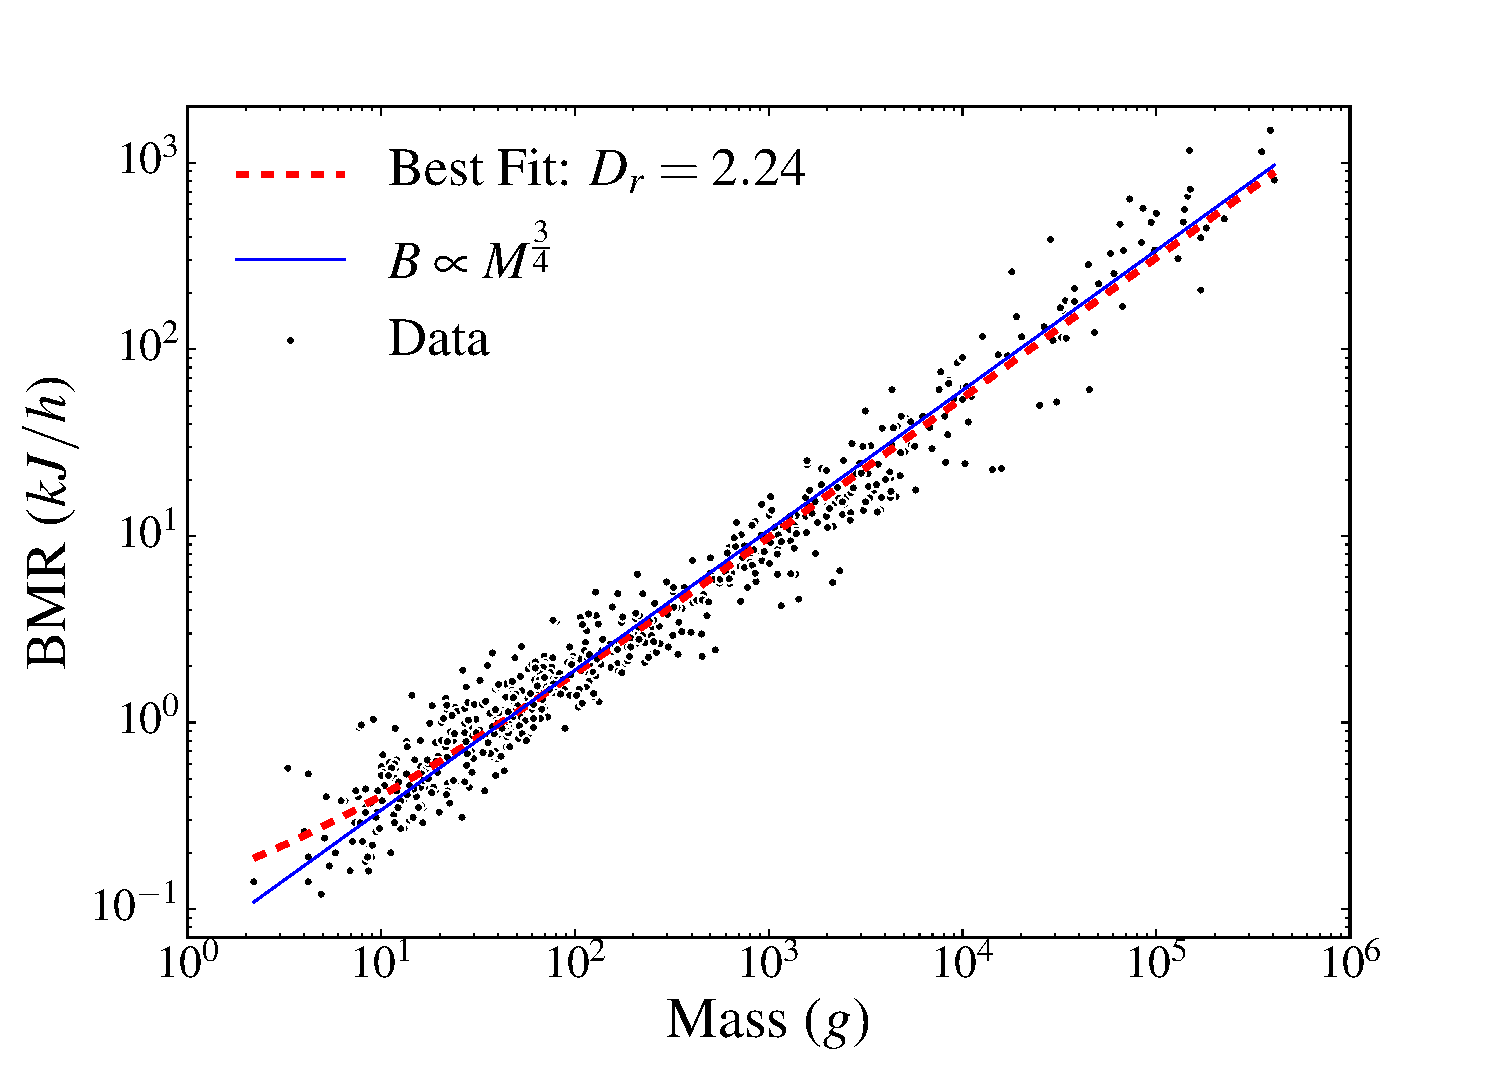
\includegraphics[height=70mm]{Figures/OrganismsPowerScaling.pdf}

<<<<<<< HEAD
  \caption{Energy-time minimization model predictions for power
    scaling in organisms. The model from Eq.~\ref{eq:OrganismPower}
    was fit to data from~\cite{kolokotrones2010curvature} by minimizing the distance
    from the empirical points to the modeled curve, similar to Reduced
    Major Axis fits. %Other minimization techniques were tested with
    %similar results (not shown). %FIXME: include an $M^{3/4}$ line for reference?
    }
=======
  \caption{Energy-time minimization model predictions for power scaling in
    organisms. The model from Eq.~\ref{eq:OrganismPower} was fit to data
    from~\cite{kolokotrones2010curvature} by minimizing the distance from the
    empirical points to the modeled curve, similar to Reduced Major Axis fits.
  Other minimization techniques were tested with similar results (not shown).
The model from \cite{west97} is included to demonstrate the curvature in the
data.}

>>>>>>> origin/master
\label{fig:OrganismsPowerScaling}
\end{figure}


The model predicts that, for the optimal network design (i.e., $D_l=3$  and
$D_r=2$), the system's energy-time product scales approximately linearly with $N$. The model is a simplification of a more complex reality. For example, although~\cite{newberry2015testing} find empirical support for the predicted $D_r \approx 2$, they do not find evidence for $D_l = 3$ in mouse vasculature, suggesting that the network is not optimally delivering resources homogenously throughout the body volume. However, even if the volume filling assumption is oversimplified, highlighting the inherent tradeoff between energy dissipation and delivery times 
%Since size increases with $N$, this suggests that the energy-time product is
%independent of body mass.
has important implications for the energetic basis of fitness.  Some have proposed that biological fitness
maximizes metabolic power (energy/time) \cite{lotka56, odum71}, whereas others
have proposed that it minimizes biological times (e.g., generation times, which
is equivalent to maximizing vital rates) \cite{lindstedt81, sibly91}. The
invariance of the energy-time product on a per-node basis is consistent with the fact that fitness
of organisms is largely independent of body mass.  Organisms of all sizes, from
small, fast, low-power microbes to large, slow, powerful mammals, coexist and,
therefore, are likely nearly equally fit.  This implies a direct trade-off
between maximizing metabolic power and minimizing generation times that holds
over the many orders of magnitude variation in body mass.  The energy-time
product reflects powerful geometric, physical and biological constraints on the
evolution of organism designs.

%This result is interesting because it provides an alternative
%explanation for area increasing branching in the circulatory system.

% Combining terms, eachARE  minimized by minimizing $D_r$.  However, $N^{-1}$
% is a lower bound on $R$ because when the summation is minimized,
% $\lambda^{-H} \propto N^{-1}$ dominates, and there is no additional benefit
% %(for the time-energy product) for $D_r < 2$.  %Because $D_l$ is 3, the
% series converges to a minimum constant value when $D_r <  3$  giving %$R
% \propto \lambda^{-H} \propto N^{-1}$.  


%in Table \ref{tab:equations}. 


\subsection{Computers}
\label{sec:computers}

We now apply the same reasoning to computer chips. 
%The energy and time relations above are valid if transistor size is kept
%constant as the system scales. In real systems, 
In computers, unlike biology, the nodes (transistors) 
%caling of transistor count is driven by reduction in feature sizes, 
are not of constant size and have shrunk by many orders of magnitude over 40
years of micro architecture evolution.  During this time, chip area has grown
much more slowly, and we assume it to be constant for our calculations.
Putting these two constraints together, the linear dimensions of transistors
and wires decrease with transistor count as $N^{-1/2}$ (more generally,
$N^{-1/D_l}$) \cite{moses08}.  This miniaturization process is well understood
and accurately described by Dennard scaling \cite{dennard74}.  
%[TODO: Review Dennard scaling]  The final energy and time formulas with the
%correction for technology scaling are shown in Table \ref{tab:equations}.
Thus, $r_0 \propto l_0 \propto N^{\frac{-1}{D_l}}$. Intuitively, this means
that the number of nodes increases as smaller transistors are placed closer
together and connected with smaller and shorter wires. In the following,
we assume that all wires carry the same flow and that information is
transferred synchronously. We now calculate how $E_{net}$, $T_{net}$,
$E_{node}$ and $T_{node}$ scale with the number of transistors, $N$, and the 3
dimensions, $D_l$, $D_r$ and $D_w$.

$E_{net}$ can be calculated from basic principles of electronics as the energy
dissipated to transmit a bit over a wire: $\frac{CV^2}{2}$, where $C$ is
capacitance and $V$ is voltage.  Because $V$ has remained approximately
constant over the last four decades (decreasing only by a factor of five while
transistor count increased by six orders of magnitude \cite{ning07}), we
estimate that the total energy to transmit all bits over the network scales as
$C$ \cite{bingham08}.  Ignoring fringe effects and for an aspect ratio of 1,
wire capacitance is proportional to wire length, $C = \epsilon l$
\cite{wilhelm95}, where $\epsilon$ is the dielectric constant. Thus, the
network capacitance is the sum of the capacitances of all wires, which is
proportional to the total wire length of the network~\cite{donath79}:

\begin{equation}
  \label{eq:ChipsEnet}
  E_{net} \propto C \propto  \sum_{i=0}^H l_i w_i n_i \propto l_0 w_0 \lambda^H
\sum_{i=0}^H \lambda^{i \left( \frac{1}{D_l} + \frac{1}{D_w} -1 \right)}
\end{equation}

\noindent where at all levels $i$, $l_i$ is the length of wire, $w_i$ is the number of wires per
module, and $n_i$ is the number of modules. Recalling that
$l_0 \propto N^{-1/D_l}$ and $\lambda^H \propto N$ gives: 
%\begin{equation}
%E_{net} \propto C \propto L_{net}
% \propto  \sum_{i=0}^H l_i w_i n_i \propto l_0 w_0 \lambda^H \sum_{i=0}^H \lambda^{i \left( \frac{1}{D_l} + \frac{1}{D_w} -1 \right)}
\begin{equation}
\label{eq:comp-Enet}
  E_{net}  \propto  N^{(1- \frac{1}{D_l})} \sum_{i=0}^H \lambda^{i \left( 
\frac{1}{D_l} + \frac{1}{D_w} -1 \right)}
\end{equation}

\noindent Note that the scaling of $E_{net} $ with $N$ depends on $D_l$ and
$D_w$, but not on $D_r$. Similarly to energy scaling in
organisms, how $E_{net}$ scales depends on whether the exponent
$\frac{1}{D_l} + \frac{1}{D_w}-1$ in Eq.~\ref {eq:comp-Enet} is positive or
negative.  If $D_w \geq \frac{D_l}{D_l -1}$ the exponent is negative and the
summand converges to a constant (or $\log(N)$ in the exact equality case),
leaving $E_{net} \propto N^{1-\frac{1}{D_l}}$. When $D_w < \frac{D_l}{D_l -1}$,
$C \propto N^{\frac{1}{D_w}}$. Given $D_l$ for 2-dimensional chips, $E_{net}$
is minimized when $D_w \geq 2$. See Section~\ref{sec:AppendixChips} for
details.

We now calculate the scaling of $E_{node}$. 
%%FIXME(should we say
%something about leakage power here, as in acknowledging that it exists
%and saying why we ignore it?) 
For a single node, computation
energy is given by the transistor's (dynamic) energy dissipation as
$\frac{CV^2}{2}$. Again assuming constant $V$ and the capacitance of a
transistor proportional to it's length ($l_0$), $E_{node}$ is obtained
by summing
the capacitance across all $N$ nodes giving $E_{node} \propto N l_0  \propto
N^{1-\frac{1}{D_l}}$. 

We calculate $T_{net}$ as the time to transmit a bit over the last logic wire
in the network that connects to each transistor. This assumes perfect
pipelining so there is no delay in bits arriving at the last wire
(Appendix~\ref{sec:AppendixChips} shows that perfect pipelining requires $D_r =
2$). Thus, $T_{net}$ is equivalent to the wire latency which equals resistance
multiplied by the capacitance of the wire ($RC$). For wires with aspect ratio
1, $R_i = \rho l_i /r_i^2$, where $\rho$ is the resistivity of the material,
and $C_i \propto l_i$ as above.  Thus, 

\begin{equation}
\label{eq:comp-Tnet}
T_{net} \propto R_0C_0 \propto
\frac{{l_0}^2}{{r_0}^2} \propto N^0
\end {equation}
\noindent $ \frac{{l_0}^2}{{r_0}^2}$ is constant
because in chips  $l_0 \propto r_0$ and both are set by process size.

Computation time for each node, $T_{node}$, is calculated as the transistor
delay, $\frac{CV}{I}$~\cite{bakoglu90}, where again $V$ is constant and $C$ is
proportional to transistor length: $T_{node} \propto C_0 \frac{V}{I}  \propto
l_0  \propto N^{-\frac{1}{D_l}}$. 

%[YIKES, what happened to $I$?]. [GEORGE
%DIDN'T INCLUDE A CALCULATION HE JUST REFERENCES~\cite{bakoglu90}].

Before calculating the energy time product, we observe that $T_{net}$ is the
only term that depends on $D_r$, so we set  $D_r = 2$ to minimize
$T_{net}$. Similarly, $E_{net}$ is the only term that depends on  $D_w$, and we
set $D_w$ to minimize $E_{net}$.  In summary, given $D_l = 2$, the terms of the energy-time product are minimized
when $D_r = 2$ and $D_w > 2$, and the scaling relations for various
quantities are shown in Table~\ref{tab:SummaryScalingPredictions}.

%FIXME(SF liked the text that is now deleted that gave a narrative
%about why the results come out like they do.)
%
%[PUT these in a table. DONE]
%
%$E_{net} \propto N^{1-1/D_l} \propto N^{1/2}$
%
%$E_{node} \propto N^{1-1/D_l} \propto N^{1/2}$
%
%$T_{net} \propto N^0$
%
%$T_{node} \propto N^{-1/D_l} \propto N^{{-1}/2}$
%
%%Thus, for 2 dimensional chips in which $D_l = 2$, three components of the
%%energy time product ($E_{net}$, $E_{node}$, and $T_{node}$) scale sub linearly
%%(as $N^{1/2}$ and $N^{-1/2})$ but $T_{net}$ is are constant with respect to $N$.
%
%
%Putting it all together, 
%
%$E_{sys} = E_{net} + E_{node}  \propto N^{1/2}$ 
%
%$T_{sys}  = max(T_{net}, T_{node}) \propto N^0$
%
%$E_{sys} \times T_{sys} \propto N^{\frac{1}{2}}$
%\subsection{Fitness Functions of Design}
%
%
%Recall that we express the system's energy is given as $E_{sys} = E_{net} + E_{node}$, 
%and the system's time as $T_{sys} = T_{net} + T_{node}$.  For 
%organisms, we write:
%
%\begin{equation}
%\begin{cases}
%\text{{\bf Minimize:}}\\
%\text{\;\;\;} E_{sys}\times T_{sys} (D_l, D_r) \propto \left( 
%N^{\frac{2}{D_r}-1} + N^0 \right) \times \left( N^{1 
%- \frac{2}{D_r}}+ N^{1 
%- \frac{2}{D_r}}\right)\\
%\,\\
%\text{{\bf Subject to:}}\\
%\text{\;\;\;} D_l = 3\text{ and } 2\leq D_r < \frac{4D_l}{1 + D_l}
%\end{cases}
%\label{eq:organism}
%\end{equation}\\
%
%and for computers:
%\begin{equation}
%\begin{cases}
%\text{{\bf Minimize:}}\\
%\text{\;\;\;} E_{sys}\times T_{sys} (D_l, D_r, D_w) \propto \left( N^{
%- \frac{1}{D_l}} + N^{- \frac{1}{D_l}}\right) \times \left( 
%  N^{\frac{2}{D_l} -\frac{2}{D_r}}  + N^{ - \frac{1}{D_l}}\right)\\
%\,\\
%\text{{\bf Subject to:}}\\
%\text{\;\;\;} D_l=2 \text{, } D_r \geq D_l \text{, and } D_w > 
%\frac{D_l}{D_l-1}.
%\end{cases}
%\label{eq:computer}
%\end{equation}\\


 
%Analysis of Equation~\ref{eq:organism} determines the optimal value of $D_r$
%for organisms. Although energy dissipated by the network decreases as $D_r$
%increases, we observe that for $D_r \geq 2$ the energy consumed by the nodes
%($N$) dominates the energy dissipated by the network ($l_0 u_0
%N^{\frac{2}{D_r} - 1}$).  Therefore, there is no additional benefit to setting
%$D_r>2$. Similarly, time is reduced by having $D_r=2$ and,
%therefore, the minimum energy-time product occurs at $D_r = 2$.  This result
%shows that 


\subsection{Predictions for Chips}
\label{sec:comp-predictions}


For computers, minimizing the energy-time product in the model is trivial: $D_l=D_r=D_w =
2$. This result corresponds to ideal scaling, as suggested by Dennard
\cite{dennard74}, where the linear dimensions of transistors and wires scale at
the same rate, wire delay is constant, and the Rent's exponent is 1/2.  Although
the energy-time product is also minimized for values of $D_w$ greater than 2,
this would entail greater communication locality, which is challenging
to engineer, and no
improvement of the energy-time product.  Thus, it is not surprising
that $D_w = 2$ which is consistent with observed
Rent's exponents that approach 1/2~\cite{yang2001wirelength}. 


The final energy-time product scales as $N^{1/2}$, showing that, unlike
organisms, as size increases, the energy-delay product per node decreases
systematically.  Thus, chips have become faster and they consume less energy per
transistor as more transistors are packed onto a chip. Of course, this
result arises 
from the remarkable miniaturization of transistors and wires described by
Moore's law. It is not surprising that transistors are faster ($T_{node}$) and
require less energy ($E_{node}$) as they become smaller. It also makes sense
that  $E_{net}$ grows sub-linearly with the number of transistors, because as
$N$ increases the distance between nodes is reduced. Additionally, $D_w = 2$,
means that most bits move locally, so the distance between nearest nodes
affects the average distance that bits are transmitted.  The only term in the
energy-time product that does not decrease with increased $N$ and decreased
process size is $T_{net}$ which remains constant under Denard scaling in which
wire radius and length scale proportionally to each other.

Our scaling models make two important predictions.  First, power
consumption in chips (total energy dissipated per unit of time) scales as

\begin{equation}
\label{eq:Power}
Power = \frac{E_{sys}}{T_{sys}} \propto N^{1/2} 
\end{equation}
 
\noindent Second, performance,
measured as computations executed per unit of time, or throughput, is predicted
to scale linearly with $N$,  i.e.  

\begin{equation}
\label{eq:Performance}
Performance\propto \frac{N}{T_{sys}} \propto N
\end{equation}
%assuming that a constant fraction of the transistors is active at each cycle, 

We compared our theoretical predictions for power consumption with data obtained for 523
different microprocessors over a range of approximately 6 orders of magnitude
in transistor count.  The data are shown in Figure~\ref{fig:power}, where the
measured exponent was $0.495$ (95\% confidence interval = 0.46 to 0.53) which agrees closely with our prediction of
$0.5$. Consistent data on performance across many technology generations is
difficult to obtain because reporting standards have changed over the years and 
adoption by different vendors is not uniform.  We were able to obtain
normalized performance data for 100 different chips Intel Chips as measured
with Dhyrstone Millions of Instructions per Second (DMIPS). This data came from
a variety of published third-party performance comparisons from different
generations over a range of 6 orders of magnitude in transistor count.  The
exponent obtained for these data is $1.11$ (95\% confidence interval =1.07 to 1.15), as shown in
Figure~\ref{fig:throughput}. This is very close to our predicted exponent of
$1$, suggesting that engineered designs slightly outperform the
theoretical optimal defined by the model.  
% SF thinks maybe the vendors are 'cheating' on the data they report.

The linear increase in performance with the number of transistors is somewhat
counter-intuitive. Given that transistor switching times have decreased
dramatically as size has decreased, one might expect performance to increase as
the product of clock speed and transistor number ($N$). This is not the case (the
predicted performance if time were the inverse of clock speed is shown in the
green dashed line in Figure~\ref{fig:throughput}). Some performance increases
are achievable by increasing clock speed for a given manufacturing process,
which may account for the higher than predicted scaling
exponent\footnote{Additionally higher end chips are more likely to be
  benchmarked, potentially leading to a bias in the data towards higher
performing chips.}. Our analysis suggests that the network is indeed
the bottleneck. The network delivers bits to transistors at a constant rate per transistor
(Eq.~\ref{eq:comp-Tnet}), so performance has increased only linearly with transistor
number even though, in principle, transistors could process information more
quickly.  As in biology, performance cannot be
understood without considering the constraints of the network.

%[Add above] Not all transistors are computing on every clock tick because transistor activity is determined by the logic that controls the computation.

%[maybe somewhere] Although resting transistors do consume power (leakage power), the data is only active power.
 


\begin{figure}[!h]
\centering
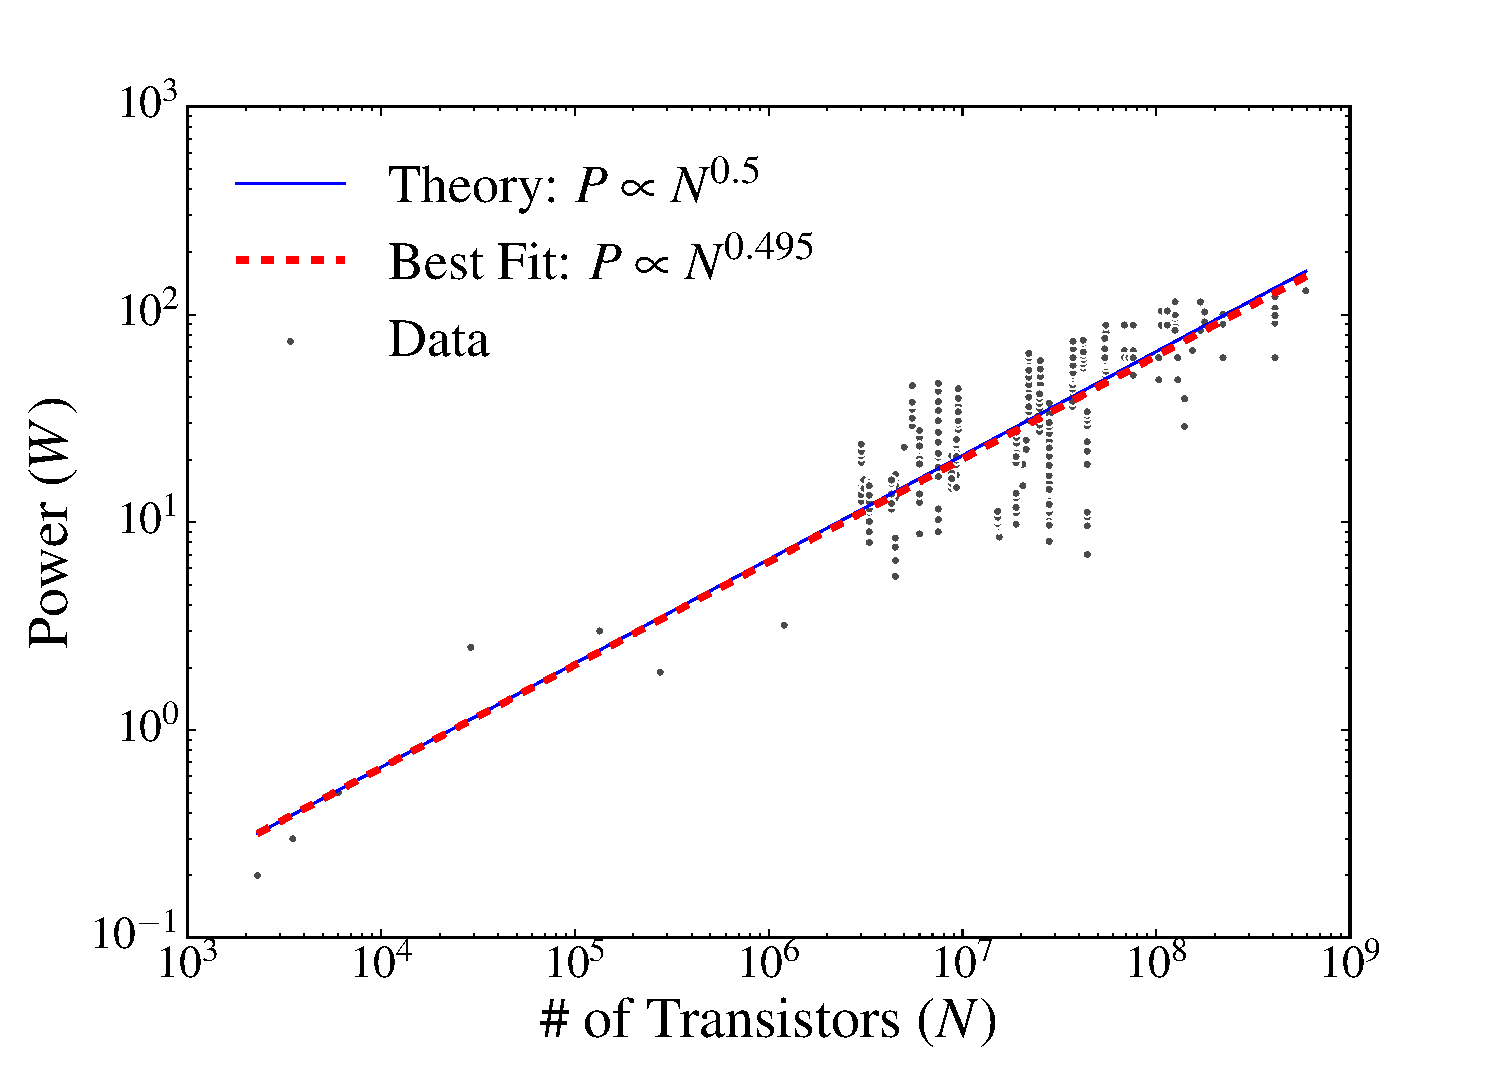
\includegraphics[height=70mm]{Figures/ChipsPowerScaling.pdf}
\caption{Power vs number of transistors predicted from Eq.~\ref{eq:Power}}
\label{fig:power}
\end{figure}

\begin{figure}[!h]
\centering
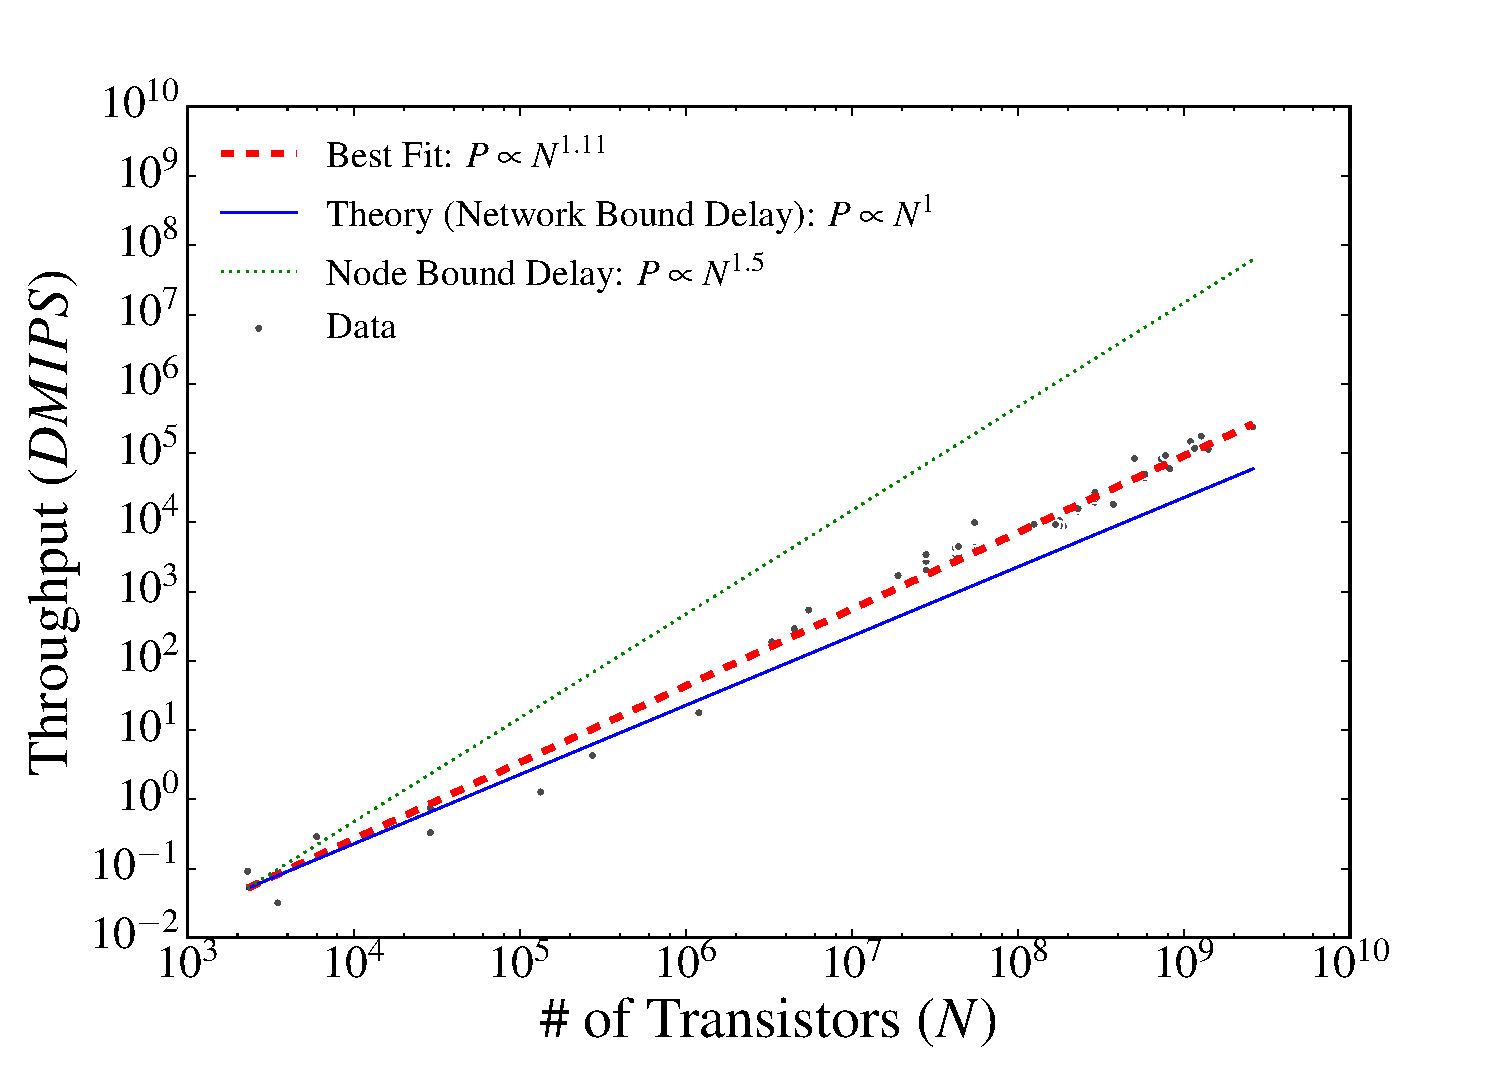
\includegraphics[height=70mm]{Figures/ChipsThroughputScaling.pdf}
\caption{Performance vs number of transistors. The prediction from Eq.~\ref{eq:Performance} that reflects the limitations of the network provides better predictions than the alternative assumption that performance is limited by the switching speed of the transistors.}
\label{fig:throughput}
\end{figure}

Our model provides a simple theoretical explanation for the scaling of power
and performance in computers over 40 years of microprocessor technology
improvements.  The excellent agreement between the theoretical optimum and
experimental data suggests that through successive generations of
trial-and-error, innovation and optimization, engineered designs are highly
successful, approaching the theoretical limit predicted by the model.

\section{Discussion: Implications for Evolutionary Transitions}
\label{sec:discussion}

Scaling analyses provide a framework for identifying invariants and
understanding constraints on both biological and computational systems over
enormous size ranges.  By simultaneously minimizing energy dissipation and delivery
time, our unified model 
%in both the network and the nodes, 
% SF not sure what delivery time in a node is.
predicts scaling relationships for both
organisms and computer chips.  This broad framework highlights the similarities
and differences between biological networks that deliver energy and
computational networks that deliver information. 

The similarities between biological and computational scaling
suggest likely future trajectories in computing based on how biology
has changed over evolutionary time. For this we turn to work by Delong et al.~\cite{delong2010shifts} who
demonstrated that metabolic scaling slopes and intercepts change at the
evolutionary transitions: prokaryote (bacteria) metabolism varies superlinearly with
size, unicellular protist metabolism varies linearly, and multicellular animal
metabolism is sublinear, converging toward the canonical $3/4$ exponent. They
hypothesize that these discontinuous shifts arise from organisms overcoming a series of
constraints, and then facing new constraints, as they increase in size.

Larger bacteria increase metabolism as additional genes allow increased use of
metabolic substrates, but eventually the cell surface area limits metabolic
processing. Unicellular protists overcome this constraint by internalizing the metabolic machinery into
respiratory organelles (i.e., mitochondria that convert oxygen into ATP). The
number of mitochondria increases linearly with cell size until internal
transport constraints begin to limit the rate of metabolic processing.
Next, multi-cellular
animals developed internal networks to speed the delivery of metabolites,
and are subject to sublinear network scaling effects. Delong et al.\ highlight the
importance of both time and energy constraints, and they note significant decreases in energetic
efficiency at each evolutionary transition when absolute measures of time and
energy increase.  The explanations that they hypothesize are directly relevant
to understanding how energy-time minimization affects the ongoing evolution of
computer hardware.

1.     Evolution of single core chips: The chip scaling we describe above shows
how time and energy dissipation have decreased while performance increased as
larger numbers of shrinking transistors have been packed onto each chip. During
this period, similar to bacterial evolution that incorporates new genes to
exploit new metabolic niches, technological innovations have emerged. For
example, new materials, switching methods, etching processes and cooling
technologies have pushed physical boundaries, allowing transistors to shrink
and more of them to be packed onto each chip. Like bacteria, these innovations
have optimized physical constraints, but there is an ultimate maximum. There
are no elephant-sized bacteria and there will be no silicon based single core
chips with quadrillions of transistors.

2.  Chips have also mimicked the linear relationship between performance and
size (Figure~\ref{fig:throughput}) seen in protists. Unicellular protists show linear increases
in metabolic rate with size as more energy processing nodes  (mitochondria) are
packed into larger cells. However, like protists, this regime will eventually end due
to physical constraints.  Our earlier analysis suggests that the
internal transport network already constrains the processing speed of the
system (i.e., $T_{net}$ constrains $T_{sys}$). Further, the requirement to
dissipate heat over a fixed surface area constrains both cells and chips. 

3. Computer chips have begun the evolutionary transition to multicore, resembling the
biological transition to multicellularity. Our unified scaling framework
suggests future scenarios for multicore chips. As the era of transistor
minimization draws to a close, adding more transistors will require increased
area, and therefore networks that span a larger area. Similarly to
multicellular organisms, we expect that as the number of cores grows, an
increasing fraction of chip power will be devoted to these ever larger 
Networks-on-Chip (NoC) connecting more cores. Larger networks will require more
power to drive them, and it will take more time to traverse them, ultimately
making time-energy minimization increasingly difficult to sustain as chips increase in
size. It is likely that the reductions in clock speed
in multi-core chips will continue as the power, footprint and cooling requirements of the network dominate chip design considerations. As networks increasingly dominate on-chip power
budgets, it is also likely that the most important advances in chip design will be in increasing
network efficiency, for example using optical networks. 


  
The differences between scaling of energy delivery in biology and information
delivery in computation also play an important role in evolutionary
transitions. In particular, on-chip computer networks have two advantages not
available to cardiovascular networks. First, technological advances have decreased
``process'' size by orders of magnitude over the last several decades,
resulting in ever smaller transistors and wires that reduce both energy and
delay in the nodes, as well as allowing the dramatic increase in the number of
transistors and wires in a given area. This reduction in process size will end
as physical limits are reached. Second, the locality of
network traffic, characterized by the Rent's exponent and $D_w$, reduces long
distance communication over computer networks. As shown above, this wire
scaling results in lower $E_{net}$ and a smaller wire footprint as $N$
increases on single core chips. This advantage will likely continue for
multi-core chips where communication, and therefore network bandwidth,
footprint and energy consumption of NOCs can be reduced by keeping
communication primarily local~\cite{bezerra2010modeling, zarkesh2010hybrid}. Communication locality
has the potential to produce more favorable scaling in multicore
computation than is achievable in multi-cellular biology.

Scaling on computer chips and other systems in which networks deliver
information rather than energy lend insights into another important
biological evolutionary transition, the transition to social animal societies.
Delong et al.\ does not address scaling relationships in animal societies.
However, sociality is an important evolutionary transition, reflected in the
ecological dominance of humans and ants, two social species whose networked
systems exchange energy and information. These social species have dispersed over vast territories across the globe and captured
<<<<<<< HEAD
extraordinary fractions of available energy ~\cite{haberl2007quantifying, holldobler1990ants}. Recent evidence suggests that ant colonies and
human societies follow similar scaling relationships as individual organisms~\cite{moses2003allometry, bettencourt2007growth, burnside2012human, hou2010energetic, waters2010allometric}. In social animal systems and networked computer systems, networks
are at least partially decentralized, for example traffic flow within cities ~\cite{samaniego2008cities} and among ant nests~\cite{flanagan2013fast}. Understanding
=======
extraordinary fractions of available energy~\cite{haberl2007quantifying, holldobler1990ants}. Recent evidence suggests that ant colonies and
human societies follow similar scaling relationships as individual organisms
FIXME(citations). In social animal systems and networked computer systems, networks
are at least partially decentralized, for example traffic flow in cities (CITE
mosessamaniego) and communication patterns in ants (CITE Noa). Understanding
>>>>>>> origin/master
how communication locality has emerged in computation may lend insights into
one of the important benefits in the transition to sociality in biology: animal
societies have escaped the constraint of the centralized distribution network
by evolving systems for decentralized and modular communication.


%FIXME: do we need to pull other text from the BEYOND Biology chapter? 



%5.     The strong similarity in the scaling of computational and biological systems results from the fundamental dependence of both systems of the number of nodes (transistors in computation and �the number of membrane-bound respiratory complexes� that synthesize ATP from oxygen) and the geometric constraints on transport distances. 



\section{Conclusion}

Our analysis provides a unifying explanation for the origin of scaling laws in
biology and computing. Despite obvious differences in form and function, the
scaling of organisms and computers is governed by the same simple principle.
By minimizing energy dissipation and the time to deliver resources, whether through natural selection or
engineering, existing designs manage the trade-off between cost and
performance, leading to general scaling patterns observed over several orders
of magnitude in size.  Moreover, power laws as a function of size are not
unique to organisms and computers but are observed across a wide
variety of complex systems in nature, society and technology.  The scaling of
white and grey matter in the brain \cite{zhang00}, of energy use and GDP in
countries \cite{brown11}, and the pace of life and population in cities
\cite{bettencourt07} are additional examples where a unifying explanation is
still lacking.  Because cost and performance, i.e., energy and time, impose
universal constraints, we suggest that a common design principle governs the
scaling of complex systems that process energy, materials and information.

Engineering ingenuity and economic pressures have created increasingly
fast and powerful computers through a series of innovations, including
integrated circuits, innovations in materials and other technological
tricks, synchronizing clock trees, multi-core chips and networked and
distributed computation. Technological evolution is undergoing another
major evolutionary transition as distributed computing changes the
metabolic landscape of technology and its interaction with the
environment. As computers become more embedded in physical devices,
physical proximity and energy concerns for low-power devices may drive
computational scaling to more closely resemble biological scaling. In
computation, dramatic changes have emerged over the last 35 years, but
to a surprising extent, their trajectories mimic the biological
transitions that took billions of years to evolve simple unicellular
bacteria into the largest and most powerful animals and societies on
earth.



%By unifying time and energy into a single model, the model accounts for the wide variation in size of organisms and computers, e.g., mouse to elephant and arm to multe-core.  
  
  

%\section{Additional Discussion point}



%\item What do we want to say about data centers?  Is this some new
%  evolutionary level?


 


%\item If we're gonna say this, we have to actually do it. I'm inclined to skip it.
%
% Our framework gives a theoretical explanation for well-known empirical patterns in computer
%  architecture.We provide an explanation for Koomey's Law (p. 13). These results also provide an explanation for Koomey's Law, which states
%roughly: ``The number of computations per joule of energy dissipated has been
%doubling approximately every 1.57 years." This follows directly from minimizing
%the energy time product and Moore's Law, the empirical observation that the
%number of transistors ($N$) doubles every 2 years. NEED a figure that combines
%data from Fig 2 and Fig 3 to show this?



%\item Nature dealt with network design constraints by slowing metabolism as
%  animal size increases.  Computer architecture, at least until recently,
%  focused on increase clock speeds by minimizing component size and incresing
%  energy per chip.  Also, using the third dimension to accommodate more wires, 

%\item Computer transitons: transistors; transistors to integrated circuits;
%  single core to multi-core; desk tops to data centers.  Multicore is an
%  evolutionary transition.  IBM currently making 10 nm chips which are the
%  limit for silicon.  IBM recently announced a 7 nm transistor (more than 1000
%  times smaller than the diameter of a red blood cell) and only three times
%  larger than a strand of DNS, using silicon germanium targeting a 50\% power
%  improvement.  NYT July 9, 2015.  Then going to carbon nanofibers. 
  
%\end{itemize}



\section{Appendix A: Details of Scaling in Organisms}
\label{sec:AppendixOrg}

In this section we give a detailed analysis of the derivation of the scaling
of the total network resistance discussed in Section~\ref{sec:organisms}, and its
subsequent effect on the energy time product scaling. Recall that $D_l = 3$
for $3$ dimensional organisms and that $\lambda^{-H}=N^{-1}$.  Using these
values and simplifying, equation~\ref{eq:resistance} is transformed. 

\begin{equation}
 R = \frac{8 \mu l_0}{\pi r_0^4} N^{-1} \sum_{i=0}^H \lambda^{i(\frac{4}{3} -\frac{4}{D_r})}
\end{equation}

Let the summand $S = \sum_{i=0}^H \lambda^{i(\frac{4}{3} -\frac{4}{D_r})}$. $R \propto
N^{-1} S$. How $S$ scales with $N$ is dependent on the exponent $\frac{4}{3} -
\frac{4}{D_r}$, and reduces to four different cases:

\begin{caseof}

    \case{$D_r=3$}{In this case the exponent is equal to 0, and the $S = H+1
      \propto \log (N)$, and $R\propto \frac{\log(N)}{N}$, because $\log(N)$
      in this case grows much more slowly than $N$, it is reasonable to
      conclude that $R\propto N^{-1}$. In this case the energy time product
      scales as $l_0 + u_0^{-1}N^{2-\frac{2}{D_r}}$.}

    \case{$D_r < 3$}{Here (and in subsequent cases) we can use the geometric
      series to calculate the exact value of $S$. In particular 

      \begin{align*}
        S &= \frac{(1-\lambda^{(\frac{4}{3}
    -\frac{4}{D_r})(H+1)})}{1-\lambda^{\frac{4}{3} -\frac{4}{D_r}}} \\ 
        &= \frac{1-\left(\lambda^{H}\right)^{(\frac{4}{3}-\frac{4}{D_r})}
      \lambda^{(\frac{4}{3} - \frac{4}{D_r}))}}{1-\lambda^{\frac{4}{3}
      -\frac{4}{D_r}}} \\
        &= \frac{1-N^{(\frac{4}{3}-\frac{4}{D_r})}
      \lambda^{(\frac{4}{3} - \frac{4}{D_r}))}}{1-\lambda^{\frac{4}{3}
           -\frac{4}{D_r}}}
      \end{align*}

      If we let $c = \lambda^{(\frac{4}{3} -\frac{4}{D_r})}$ we see that

      \begin{equation}
        S = \frac{1-c N^{(\frac{4}{3}-\frac{4}{D_r})}}{1-c}
      \end{equation}

      Because $\frac{4}{3} - \frac{4}{D_r} < 0$ is negative in this case
      and $N$ is large in practice, $c N^{(\frac{4}{3} -\frac{4}{D_r})}$ is
      small, and $S$ is proportional to a constant ($S \approx
    \frac{1}{1-c}$). This implies that $R \propto N^{-1}$. Once
  again~\ref{eq:TheWholeEnchilada} scales as $\propto l_0 +
u_0^{-1}N^{2-\frac{2}{D_r}}$.}

    \case{$3 < D_r < 12 $}{In this case the exponent in $S$ is positive,
      meaning that $S$ scales directly with $N$. Note that $c>1$ in this case
      and we can write 
      \begin{equation}
        S = \frac{c N^{(\frac{4}{3}-\frac{4}{D_r})}-1}{c-1}
      \end{equation}

      \noindent This means that $S \propto N^{(\frac{4}{3} - \frac{4}{D_r})}$.
      This implies that $R \propto N^{-1} S \propto N^{(\frac{1}{3}
      -\frac{4}{D_r})}$. This means that resistance still scales inversely with
      size, but at a faster rate than if $D_r \leq 3$. This implies the energy
    time produce scales as $\propto N^{\frac{4}{3} - \frac{4}{D_r}} +
  N^{2-\frac{2}{D_r}}$.}

   \case{$D_r \geq 12$}{This final case is analogous to the one above, except
   that now resistance scales positively with $N$, implying that the energy in
 the network would scale positively with $N$. This is likely a non-physical
 possibility, but we include it here for completeness.}

\end{caseof}

\section{Appendix B: Details of Scaling in Electronics}
\label{sec:AppendixChips}

In this section we give a detailed analysis of the derivation of the scaling of
the network capacitance and network latency discussed in
Section~\ref{sec:computers}.

\subsection{Capacitance}

Recall that $D_l = 2$ for $2$ dimensional computer
chips and that $\lambda^{-H}=N^{-1}$. We can then calculate capacitance as:

\begin{equation}
  C \propto  N^{(1- \frac{1}{D_l}} \sum_{i=0}^H \lambda^{i \left( 
\frac{1}{D_l} + \frac{1}{D_w} -1 \right)}
\end{equation}

Similar to how we handled organsims we are interested in whether the exponent
$\frac{1}{D_l} + \frac{1}{D_w} -1$ is positive or negative.

Let the summand $S = \sum_{i=0}^H \lambda^{i(\frac{1}{D_l} +
\frac{1}{D_w}-1)}$. $C \propto
N^{1-\frac{1}{D_l}} S$. 

\begin{caseof}

  \case{$D_r=\frac{D_l}{D_l-1}$}{In this case the exponent is equal to 0, and the $S = H+1
    \propto \log (N)$, and $C\propto \log(N) N^{1-\frac{1}{D_l}}$, because $\log(N)$ in
    this case grows much more slowly than $N^{1-\frac{1}{D_l}}$ and we know
    $D_l=2$ for 2 dimensional chips, it is reasonable to conclude that
  $C\propto N^{\frac{1}{2}}$}

  \case{$D_r > \frac{D_l}{D_l-1}$}{Here (and in subsequent cases) we can use
    the geometric series to calculate the exact value of $S$, using a similar
  approach to~\ref{sec:AppendixOrg}. In this case the exponent is negative and $S$
is a small constant, leaving $C \propto N^{\frac{1}{2}}$}

\case{$D_r < \frac{D_l}{D_l-1} $}{In this case the exponent in $S$ is positive,
      meaning that $S$ scales directly with $N$. Now the summand contributes an
    $N^{\frac{1}{D_l}+\frac{1}{D_w} -1}$ and $C \propto N^{\frac{1}{D_w}}$.}

\end{caseof}

\subsection{Network Delay}

Recall that we wish to determine the network latency $L$ which is defined as:

\begin{equation}
  T_{net} \propto \max_{i} L_i
\end{equation}

\noindent with

\begin{equation}
  L_i \propto RC = \frac{\rho \epsilon li^2}{r_i^2} = \frac{\rho \epsilon
  l_0^2}{r_0^2} \lambda^{i\left(\frac{2}{D_l} - \frac{2}{D_r}\right)}
\end{equation}

\noindent $L_i$ will scale differently depending on the relative values of
$D_r$ and $D_l$. 

\begin{caseof}

  \case{$D_r>D_l$}{In this case the fraction in the exponent is greater than 0
  and the latency will be highest when $i=H$, resulting in $L \propto
N^{\frac{2}{D_l} - \frac{2}{D_r}}$. }
  
  \case{$D_r <  D_l$}{In this case the exponent is negative and the highest
  latency occurs at the bottom of the network $i=0$, leaving $L\propto
\frac{l_0^2}{r_0^2} \propto N^0$}

  \case{$D_r = D_l$}{In this case the exponent is 0 and there is equal latency
  at all levels and $L \propto N^0$.}
\end{caseof}

<<<<<<< HEAD
%\newpage
%\begin{table}
%\centering
%\begin{tabular}{|l|l|l|l|l|}
%\hline
%\multicolumn{2}{|l|}{} & $D_r=2$ & $2<D_r\leq 3$ & $Dr>3$ \\
%\hline
%\multirow{2}{*}{$E_{net}$} & Organisms & $l_0 u_0$ &$l_0u_0 N^{\frac{2}{D_r}-1}$ &$l_0 u_0 N^{\frac{1}{3} - \frac{2}{D_r}}$ \\
%\cline{2-5}
%& Computers & $N^{\frac{1}{2}}$& $N^{\frac{1}{2}}$& $N^{\frac{1}{2}}$\\
%\hline
%\multirow{2}{*}{$E_{node}$} & Organisms &  N & N  & N \\
%\cline{2-5}
%& Computers & $N^{\frac{1}{2}}$&$N^{\frac{1}{2}}$ &$N^{\frac{1}{2}}$ \\
%\hline
%\multirow{2}{*}{$T_{net}$} & Organisms & $u_0^{-1}$ & $u_0^{-1}N^{1-\frac{2}{D_r}}$ &$u_0^{-1} N^{1-\frac{2}{D_r}}$ \\
%\cline{2-5}
%& Computers & $N^{0}$& $N^{0}$& $N^{0}$\\
%\hline
%\multirow{2}{*}{$T_{node}$} & Organisms & $u_0^{-1}$ & $u_0^{-1}N^{1-\frac{2}{D_r}}$ &$u_0^{-1} N^{1-\frac{2}{D_r}}$ \\
%\cline{2-5}
%& Computers & $N^{-\frac{1}{2}}$& $N^{-\frac{1}{2}}$& $N^{-\frac{1}{2}}$\\
%\hline
%\multirow{2}{*}{$E_{sys} \times T_{sys}$} & Organisms & $l_0 + u_0^{-1} N$ &$l_0 + u_0^{-1}N^{2-\frac{2}{D_r}}$ &$l_0 N^{\frac{4}{3} - \frac{4}{D_r}} + u_0^{-1}N^{2-\frac{2}{D_r}}$ \\
%\cline{2-5}
%& Computers & $N^{\frac{1}{2}} + N^{\frac{1}{2}}$&$N^{\frac{1}{2}} + N^{\frac{1}{2}}$ &$N^{\frac{1}{2}} + N^{\frac{1}{2}}$ \\
%\hline
%\multirow{2}{*}{$\frac{E_{sys}}{T_{sys}}$} & Organisms &$l_0 u_0^2 + u_0 N$ &$l_0u_0^2 N^{2-\frac{4}{D_r}} + u_0 N^{\frac{2}{D_r}}$ & $l_0 u_0^2 N^{-\frac{2}{3}} + u_0 N^{\frac{2}{D_r}}$\\
%\cline{2-5}
%& Computers &$N^{\frac{1}{2}} + N^{\frac{1}{2}}$ &$N^{\frac{1}{2}} + N^{\frac{1}{2}}$ &$N^{\frac{1}{2}} + N^{\frac{1}{2}}$ \\
%\hline
%\multirow{2}{*}{$\frac{N}{T_{sys}}$} & Organisms &NA &NA & NA\\
%\cline{2-5}
%& Computers &$N$ &$N$ &$N$ \\
%\hline
%
%\end{tabular}
%\caption{Scaling relationships for various values of $D_r$.FIXME: this table should probably be cut? Or at least reorganized.\label{tab:CompleteScalingPredictions}}
%\end{table}
=======
\newpage
\begin{table}
\centering
\begin{tabular}{|l|l|l|l|l|}
\hline
\multicolumn{2}{|l|}{} & $D_r=2$ & $2<D_r\leq 3$ & $Dr>3$ \\
\hline
\multirow{2}{*}{$E_{net}$} & Organisms & $l_0 u_0$ &$l_0u_0 N^{\frac{2}{D_r}-1}$ &$l_0 u_0 N^{\frac{1}{3} - \frac{2}{D_r}}$ \\
\cline{2-5}
& Computers & $N^{\frac{1}{2}}$& $N^{\frac{1}{2}}$& $N^{\frac{1}{2}}$\\
\hline
\multirow{2}{*}{$E_{node}$} & Organisms &  $N$ & $N$  & $N$ \\
\cline{2-5}
& Computers & $N^{\frac{1}{2}}$&$N^{\frac{1}{2}}$ &$N^{\frac{1}{2}}$ \\
\hline
\multirow{2}{*}{$T_{net}$} & Organisms & $u_0^{-1}$ & $u_0^{-1}N^{1-\frac{2}{D_r}}$ &$u_0^{-1} N^{1-\frac{2}{D_r}}$ \\
\cline{2-5}
& Computers & $N^{0}$& $N^{0}$& $N^{0}$\\
\hline
\multirow{2}{*}{$T_{node}$} & Organisms & $u_0^{-1}$ & $u_0^{-1}N^{1-\frac{2}{D_r}}$ &$u_0^{-1} N^{1-\frac{2}{D_r}}$ \\
\cline{2-5}
& Computers & $N^{-\frac{1}{2}}$& $N^{-\frac{1}{2}}$& $N^{-\frac{1}{2}}$\\
\hline
\multirow{2}{*}{$E_{sys} \times T_{sys}$} & Organisms & $l_0 + u_0^{-1} N$ &$l_0 + u_0^{-1}N^{2-\frac{2}{D_r}}$ &$l_0 N^{\frac{4}{3} - \frac{4}{D_r}} + u_0^{-1}N^{2-\frac{2}{D_r}}$ \\
\cline{2-5}
& Computers & $N^{\frac{1}{2}} + N^{\frac{1}{2}}$&$N^{\frac{1}{2}} + N^{\frac{1}{2}}$ &$N^{\frac{1}{2}} + N^{\frac{1}{2}}$ \\
\hline
\multirow{2}{*}{$\frac{E_{sys}}{T_{sys}}$} & Organisms &$l_0 u_0^2 + u_0 N$ &$l_0u_0^2 N^{2-\frac{4}{D_r}} + u_0 N^{\frac{2}{D_r}}$ & $l_0 u_0^2 N^{-\frac{2}{3}} + u_0 N^{\frac{2}{D_r}}$\\
\cline{2-5}
& Computers &$N^{\frac{1}{2}} + N^{\frac{1}{2}}$ &$N^{\frac{1}{2}} + N^{\frac{1}{2}}$ &$N^{\frac{1}{2}} + N^{\frac{1}{2}}$ \\
\hline
\multirow{2}{*}{$\frac{N}{T_{sys}}$} & Organisms &NA &NA & NA\\
\cline{2-5}
& Computers &$N$ &$N$ &$N$ \\
\hline

\end{tabular}
\caption{Scaling relationships for various values of $D_r$.FIXME: this table should probably be cut? Or at least reorganized.\label{tab:CompleteScalingPredictions}}
\end{table}
>>>>>>> origin/master

\newpage

\bibliography{references}
\bibliographystyle{abbrv}

%\newpage
%
%\section*{Figure legends}
%\paragraph{Figure 1:} Log-log plot of power consumption as a function 
%of transistor count for 523 computer microprocessors from different 
%vendors and technological generations.  The linear regression slope is 
%$0.495$ with correlation coefficient of $0.81$. A regression that 
%removes the first seven data points and focuses on the main cloud of 
%more modern chips produces a slope of $0.487$.
%
%\paragraph{Figure 2:} Log-log plot of normalized throughput as a 
%function of transistor count for 16 Intel microprocessors from 
%different technological generations.  The linear regression slope is 
%1.0 with correlation coefficient of 0.97.

\end{document}



